\chapter{Analýza výsledkov} \label{cha:evaluation}

Táto kapitola je zameraná na detailnejšiu analýzu doposiaľ dosiahnutých výsledkov. Našim cieľom je zdôvodniť relatívne vysokú chybu (EER = $25{,}78\,\%$) ktorú dosahujú nami navrhnuté prístupy, a zistiť, či je v~tejto oblasti priestor na potenciálne zlepšenie. 

Analýzu vykonáme nad hodnoteniami výslovnosti určenými vybranou metódou, ktorej EER bola spomedzi ostatných najnižšia. Aby sme lepšie pochopili, čo je dôvodom nesprávneho hodnotenia pri tejto metóde, vyhodnotíme výsledky podľa jednotlivých foném, pri ktorých rečníci najčastejšie chybovali. Na záver podrobíme analýze aj samotný dataset nenatívnej reči, ktorý môže mať významný podiel na výslednej chybe.

\section{Vyhodnotenie výsledkov podľa foném}

Chyby u~nenatívnych rečníkov sa pri niektorých kanonických fonémach vyskytujú častejšie ako u~iných. Zároveň pri rôznych fonémach môžeme pozorovať chyby odlišného charakteru. Je pre to namieste, aby sme sa aj pri vyhodnocovaní detekcie nesprávnej výslovnosti zamerali na jednotlivé fonémy. 

K~tomuto experimentu využijeme LR GOP metódu využívajúcu vierohodnosti HMM stavov, ktoré sú určené multilingválnym (EN\,$\rightarrow$\,DE\,$\rightarrow$\,IT\,$\rightarrow$\,NN-EN) trifónovým akustickým modelom. Rovnako ako v~predchádzajúcej kapitole budeme vyhodnocovať úspešnosť pomocou EER a ROC krivky. 

Výsledky pre päť foném, pri ktorých rečníci v~testovacej sade najviac chybovali, 
sú uvedené v~tabuľke \ref{tab:eer-per-phoneme} a obrázku \ref{fig:det-per-phone}. 
Už na prvý pohľad je zrejmé, že úspešnosť pri jednotlivých fonémach je výrazne odlišná. Pri fonéme /\textipa{@}/ je EER na úrovni $34{,}52\,\%$, čo je rozdiel $14{,}01$ percentuálnych bodov oproti fonéme /\textipa{t}/. Tento výsledok je dosť prekvapivý, nakoľko bol v~tomto prípade klasifikátor trénovaný na väčšom množstve dát ako pri fonéme /\textipa{t}/. Príčin takto nízkej úspešnosti môže byť celá rada. My sa domnievame, že najvýznamnejším faktorom môže byť široká variabilita vo výslovnosti fonémy /\textipa{@}/ oproti fonéme /\textipa{t}/. Tá totiž môže spôsovať problematické rozoznanie nesprávnej výslovnosti od správnej. A~to nie len klasifikátorom, ale aj samotnými anotátormi, ktorý zabezpečovali prepis nenatívnej reči. Preto sa v~ďalšej sekcii zameriame na analýzu anotácii v~nenatívnom datasete.


\begin{table}[ht!]
    \centering
    \begin{tabular}{@{}llll@{}}
        \toprule
        \multicolumn{1}{c}{\multirow{2}{*}{Fonéma}} & \multicolumn{2}{c}{Výskyt {[}\%{]}}                                       & \multicolumn{1}{c}{\multirow{2}{*}{EER {[}\%{]}}} \\
        \multicolumn{1}{c}{}                        & \multicolumn{1}{c}{Testovacia sada} & \multicolumn{1}{c}{Trénovacia sada} & \multicolumn{1}{c}{}                              \\ \midrule
        \textipa{@}                                          & $13{,}52$                               & $16{,}88$                               & $34{,}52$                                             \\
        \textipa{I}                                          & $9{,}98$                                & $12{,}79$                               & $34{,}27$                                             \\
        \textipa{t}                                           & $7{,}84$                                & $4{,}30$                                & $20{,}51$                                             \\
        \textipa{D}                                          & $6{,}92$                                & $6{,}53$                                & $37{,}21$                                             \\
        \textipa{r}                                           & $6{,}52$                                & $3{,}58$                                & $32{,}10$                                             \\ \bottomrule
        \end{tabular}
    \caption{Výsledky dosiahnuté pre päť najviac chybovaných foném v~testovacej sade pri použití LR GOP metódy s~najlepšími výsledkami.} \label{tab:eer-per-phoneme}
\end{table}

\begin{figure}[ht!]
    \centering
    % This file was created by matplotlib2tikz v0.6.18.
\begin{tikzpicture}

\begin{axis}[
tick align=outside,
tick pos=left,
x grid style={white!69.01960784313725!black},
xlabel={FRR [\%]},
xmin=0, xmax=75,
y grid style={white!69.01960784313725!black},
ylabel={FAR [\%]},
ymin=0, ymax=75,
legend pos=north east,
%width=12.75cm,
%height=9.75cm,
legend cell align={left},
]

\addplot [semithick, blue]
table {%
0 100
0 99.7023809523809
0 99.4047619047619
0.0668002672010688 99.4047619047619
0.0668002672010688 97.0238095238095
0.200400801603206 97.0238095238095
0.200400801603206 96.4285714285714
0.267201068804275 96.4285714285714
0.267201068804275 96.1309523809524
0.334001336005344 96.1309523809524
0.334001336005344 94.9404761904762
0.467601870407482 94.9404761904762
0.467601870407482 94.6428571428571
0.53440213760855 94.6428571428571
0.53440213760855 93.4523809523809
0.868403473613894 93.4523809523809
0.868403473613894 93.1547619047619
1.26920507682031 93.1547619047619
1.26920507682031 92.5595238095238
1.33600534402138 92.5595238095238
1.33600534402138 91.9642857142857
1.40280561122244 91.9642857142857
1.40280561122244 91.3690476190476
1.60320641282565 91.3690476190476
1.60320641282565 91.0714285714286
1.73680694722779 91.0714285714286
1.73680694722779 90.7738095238095
1.80360721442886 90.7738095238095
1.80360721442886 90.4761904761905
1.937207748831 90.4761904761905
1.937207748831 90.1785714285714
2.07080828323313 90.1785714285714
2.07080828323313 89.5833333333333
2.33800935203741 89.5833333333333
2.33800935203741 88.6904761904762
2.47160988643955 88.6904761904762
2.47160988643955 88.3928571428571
2.80561122244489 88.3928571428571
2.80561122244489 88.0952380952381
2.93921175684703 88.0952380952381
2.93921175684703 87.7976190476191
3.27321309285237 87.7976190476191
3.27321309285237 87.5
3.34001336005344 87.5
3.34001336005344 86.9047619047619
3.60721442885772 86.9047619047619
3.60721442885772 86.6071428571429
3.87441549766199 86.6071428571429
3.87441549766199 86.3095238095238
4.00801603206413 86.3095238095238
4.00801603206413 85.7142857142857
4.14161656646627 85.7142857142857
4.14161656646627 85.1190476190476
4.34201736806947 85.1190476190476
4.34201736806947 84.8214285714286
4.47561790247161 84.8214285714286
4.47561790247161 84.5238095238095
4.74281897127589 84.5238095238095
4.74281897127589 83.3333333333333
4.87641950567802 83.3333333333333
4.87641950567802 82.7380952380952
5.01002004008016 82.7380952380952
5.01002004008016 82.4404761904762
5.27722110888444 82.4404761904762
5.27722110888444 81.25
5.3440213760855 81.25
5.3440213760855 80.6547619047619
5.47762191048764 80.6547619047619
5.47762191048764 80.3571428571429
5.54442217768871 80.3571428571429
5.54442217768871 79.4642857142857
5.67802271209085 79.4642857142857
5.67802271209085 79.1666666666667
6.34602538410154 79.1666666666667
6.34602538410154 78.8690476190476
6.54642618570474 78.8690476190476
6.54642618570474 78.5714285714286
6.61322645290581 78.5714285714286
6.61322645290581 78.2738095238095
6.94722778891116 78.2738095238095
6.94722778891116 77.6785714285714
7.48162992651971 77.6785714285714
7.48162992651971 77.3809523809524
7.88243152972612 77.3809523809524
7.88243152972612 77.0833333333333
8.48363393453574 77.0833333333333
8.48363393453574 76.4880952380952
8.81763527054108 76.4880952380952
8.81763527054108 76.1904761904762
8.95123580494322 76.1904761904762
8.95123580494322 75.8928571428571
9.15163660654643 75.8928571428571
9.15163660654643 75.5952380952381
9.21843687374749 75.5952380952381
9.21843687374749 75.2976190476191
9.75283901135605 75.2976190476191
9.75283901135605 75
10.0868403473614 75
10.0868403473614 74.7023809523809
10.4876419505678 74.7023809523809
10.4876419505678 74.4047619047619
10.688042752171 74.4047619047619
10.688042752171 74.1071428571429
10.7548430193721 74.1071428571429
10.7548430193721 73.8095238095238
10.8216432865731 73.8095238095238
10.8216432865731 73.5119047619048
10.9552438209753 73.5119047619048
10.9552438209753 73.2142857142857
11.0220440881764 73.2142857142857
11.0220440881764 72.3214285714286
11.8236472945892 72.3214285714286
11.8236472945892 72.0238095238095
11.8904475617902 72.0238095238095
11.8904475617902 71.7261904761905
11.9572478289913 71.7261904761905
11.9572478289913 71.4285714285714
12.0908483633935 71.4285714285714
12.0908483633935 70.8333333333333
12.4248496993988 70.8333333333333
12.4248496993988 70.5357142857143
12.625250501002 70.5357142857143
12.625250501002 70.2380952380952
12.6920507682031 70.2380952380952
12.6920507682031 69.9404761904762
12.8256513026052 69.9404761904762
12.8256513026052 69.6428571428571
12.9592518370073 69.6428571428571
12.9592518370073 69.0476190476191
13.2932531730127 69.0476190476191
13.2932531730127 68.4523809523809
13.4268537074148 68.4523809523809
13.4268537074148 68.1547619047619
14.0280561122244 68.1547619047619
14.0280561122244 67.8571428571429
14.2952571810287 67.8571428571429
14.2952571810287 67.2619047619048
14.3620574482298 67.2619047619048
14.3620574482298 66.9642857142857
14.562458249833 66.9642857142857
14.562458249833 66.3690476190476
14.6292585170341 66.3690476190476
14.6292585170341 66.0714285714286
14.7628590514362 66.0714285714286
14.7628590514362 65.7738095238095
14.9632598530394 65.7738095238095
14.9632598530394 65.4761904761905
15.497661990648 65.4761904761905
15.497661990648 64.8809523809524
15.564462257849 64.8809523809524
15.564462257849 64.2857142857143
16.0988643954576 64.2857142857143
16.0988643954576 63.6904761904762
16.2992651970608 63.6904761904762
16.2992651970608 63.0952380952381
16.4328657314629 63.0952380952381
16.4328657314629 62.797619047619
17.50167000668 62.797619047619
17.50167000668 62.5
17.7688710754843 62.5
17.7688710754843 62.202380952381
17.8356713426854 62.202380952381
17.8356713426854 61.9047619047619
18.2364729458918 61.9047619047619
18.2364729458918 61.6071428571429
18.3032732130929 61.6071428571429
18.3032732130929 61.0119047619048
18.3700734802939 61.0119047619048
18.3700734802939 60.4166666666667
18.9044756179025 60.4166666666667
18.9044756179025 60.1190476190476
18.9712758851035 60.1190476190476
18.9712758851035 59.8214285714286
19.0380761523046 59.8214285714286
19.0380761523046 59.5238095238095
19.1048764195057 59.5238095238095
19.1048764195057 59.2261904761905
19.1716766867067 59.2261904761905
19.1716766867067 58.9285714285714
19.3052772211089 58.9285714285714
19.3052772211089 58.3333333333333
19.7060788243153 58.3333333333333
19.7060788243153 58.0357142857143
19.7728790915164 58.0357142857143
19.7728790915164 57.1428571428571
19.9732798931196 57.1428571428571
19.9732798931196 56.8452380952381
20.0400801603206 56.8452380952381
20.0400801603206 55.952380952381
20.1068804275217 55.952380952381
20.1068804275217 55.6547619047619
21.0420841683367 55.6547619047619
21.0420841683367 55.3571428571429
21.1088844355377 55.3571428571429
21.1088844355377 55.0595238095238
21.1756847027388 55.0595238095238
21.1756847027388 54.7619047619048
21.8436873747495 54.7619047619048
21.8436873747495 54.1666666666667
21.9104876419506 54.1666666666667
21.9104876419506 53.5714285714286
22.1108884435538 53.5714285714286
22.1108884435538 53.2738095238095
22.2444889779559 53.2738095238095
22.2444889779559 52.9761904761905
22.5116900467602 52.9761904761905
22.5116900467602 52.6785714285714
22.7788911155645 52.6785714285714
22.7788911155645 52.0833333333333
23.0460921843687 52.0833333333333
23.0460921843687 51.7857142857143
23.1128924515698 51.7857142857143
23.1128924515698 51.4880952380952
23.1796927187709 51.4880952380952
23.1796927187709 50.8928571428571
23.5136940547762 50.8928571428571
23.5136940547762 50.5952380952381
23.6472945891784 50.5952380952381
23.6472945891784 50.297619047619
23.9812959251837 50.297619047619
23.9812959251837 49.702380952381
24.0480961923848 49.702380952381
24.0480961923848 49.4047619047619
24.1148964595858 49.4047619047619
24.1148964595858 49.1071428571429
24.1816967267869 49.1071428571429
24.1816967267869 48.8095238095238
24.248496993988 48.8095238095238
24.248496993988 48.5119047619048
24.315297261189 48.5119047619048
24.315297261189 48.2142857142857
24.5156980627923 48.2142857142857
24.5156980627923 47.9166666666667
24.9164996659987 47.9166666666667
24.9164996659987 47.6190476190476
25.3841015364061 47.6190476190476
25.3841015364061 47.3214285714286
25.7181028724115 47.3214285714286
25.7181028724115 47.0238095238095
25.9185036740147 47.0238095238095
25.9185036740147 46.7261904761905
26.185704742819 46.7261904761905
26.185704742819 46.4285714285714
26.4529058116232 46.4285714285714
26.4529058116232 46.1309523809524
26.8537074148297 46.1309523809524
26.8537074148297 45.5357142857143
27.0541082164329 45.5357142857143
27.0541082164329 45.2380952380952
27.1209084836339 45.2380952380952
27.1209084836339 44.3452380952381
27.187708750835 44.3452380952381
27.187708750835 43.75
27.7889111556446 43.75
27.7889111556446 43.1547619047619
27.8557114228457 43.1547619047619
27.8557114228457 42.8571428571429
27.9893119572478 42.8571428571429
27.9893119572478 42.5595238095238
28.0561122244489 42.5595238095238
28.0561122244489 42.2619047619048
28.3233132932532 42.2619047619048
28.3233132932532 41.9642857142857
28.4569138276553 41.9642857142857
28.4569138276553 41.6666666666667
29.3253173012692 41.6666666666667
29.3253173012692 41.3690476190476
29.5257181028724 41.3690476190476
29.5257181028724 40.7738095238095
29.7929191716767 40.7738095238095
29.7929191716767 40.4761904761905
29.9933199732799 40.4761904761905
29.9933199732799 39.8809523809524
30.060120240481 39.8809523809524
30.060120240481 39.5833333333333
30.126920507682 39.5833333333333
30.126920507682 39.2857142857143
30.2605210420842 39.2857142857143
30.2605210420842 38.6904761904762
30.3273213092852 38.6904761904762
30.3273213092852 38.0952380952381
30.8617234468938 38.0952380952381
30.8617234468938 37.797619047619
31.062124248497 37.797619047619
31.062124248497 37.5
31.1289245156981 37.5
31.1289245156981 37.202380952381
31.2625250501002 37.202380952381
31.2625250501002 36.3095238095238
31.7301269205077 36.3095238095238
31.7301269205077 35.7142857142857
31.8637274549098 35.7142857142857
31.8637274549098 35.1190476190476
32.1977287909152 35.1190476190476
32.1977287909152 34.8214285714286
32.3313293253173 34.8214285714286
32.3313293253173 34.5238095238095
32.3981295925184 34.5238095238095
32.3981295925184 33.9285714285714
32.999331997328 33.9285714285714
32.999331997328 33.6309523809524
33.0661322645291 33.6309523809524
33.0661322645291 32.7380952380952
33.1329325317301 32.7380952380952
33.1329325317301 32.4404761904762
33.4001336005344 32.4404761904762
33.4001336005344 31.25
33.5337341349365 31.25
33.5337341349365 30.952380952381
34.4689378757515 30.952380952381
34.4689378757515 30.6547619047619
34.8029392117568 30.6547619047619
34.8029392117568 30.3571428571429
35.3373413493654 30.3571428571429
35.3373413493654 30.0595238095238
35.8049432197729 30.0595238095238
35.8049432197729 29.7619047619048
36.0721442885772 29.7619047619048
36.0721442885772 29.4642857142857
36.87374749499 29.4642857142857
36.87374749499 28.5714285714286
38.0093520374081 28.5714285714286
38.0093520374081 28.2738095238095
38.7441549766199 28.2738095238095
38.7441549766199 27.9761904761905
38.9445557782231 27.9761904761905
38.9445557782231 27.0833333333333
40.748162992652 27.0833333333333
40.748162992652 26.7857142857143
41.0153640614562 26.7857142857143
41.0153640614562 26.4880952380952
41.4829659318637 26.4880952380952
41.4829659318637 25.8928571428571
41.5497661990648 25.8928571428571
41.5497661990648 25.5952380952381
41.9505678022712 25.5952380952381
41.9505678022712 25.297619047619
42.0841683366733 25.297619047619
42.0841683366733 25
42.6185704742819 25
42.6185704742819 24.702380952381
42.685370741483 24.702380952381
42.685370741483 24.4047619047619
43.0193720774883 24.4047619047619
43.0193720774883 24.1071428571429
43.1529726118904 24.1071428571429
43.1529726118904 23.8095238095238
43.2865731462926 23.8095238095238
43.2865731462926 23.5119047619048
43.5537742150969 23.5119047619048
43.5537742150969 23.2142857142857
43.8877755511022 23.2142857142857
43.8877755511022 22.9166666666667
44.4221776887108 22.9166666666667
44.4221776887108 22.6190476190476
45.1569806279225 22.6190476190476
45.1569806279225 22.3214285714286
45.2237808951236 22.3214285714286
45.2237808951236 22.0238095238095
45.7581830327321 22.0238095238095
45.7581830327321 21.7261904761905
45.8249832999332 21.7261904761905
45.8249832999332 21.4285714285714
46.4929859719439 21.4285714285714
46.4929859719439 21.1309523809524
47.0941883767535 21.1309523809524
47.0941883767535 20.8333333333333
47.6285905143621 20.8333333333333
47.6285905143621 20.5357142857143
48.6973947895792 20.5357142857143
48.6973947895792 20.2380952380952
49.8329993319973 20.2380952380952
49.8329993319973 19.9404761904762
50.501002004008 19.9404761904762
50.501002004008 19.6428571428571
50.7682030728123 19.6428571428571
50.7682030728123 19.3452380952381
50.9018036072144 19.3452380952381
50.9018036072144 19.047619047619
51.1022044088176 19.047619047619
51.1022044088176 18.75
51.5698062792251 18.75
51.5698062792251 18.452380952381
52.6386105544422 18.452380952381
52.6386105544422 18.1547619047619
53.3066132264529 18.1547619047619
53.3066132264529 17.8571428571429
54.5758183032732 17.8571428571429
54.5758183032732 17.5595238095238
54.7762191048764 17.5595238095238
54.7762191048764 17.2619047619048
54.8430193720775 17.2619047619048
54.8430193720775 16.9642857142857
54.9098196392786 16.9642857142857
54.9098196392786 16.6666666666667
55.6446225784903 16.6666666666667
55.6446225784903 16.0714285714286
55.7114228456914 16.0714285714286
55.7114228456914 15.7738095238095
55.8450233800935 15.7738095238095
55.8450233800935 15.1785714285714
56.8470273881096 15.1785714285714
56.8470273881096 14.8809523809524
57.3814295257181 14.8809523809524
57.3814295257181 14.5833333333333
57.4482297929192 14.5833333333333
57.4482297929192 14.2857142857143
57.8490313961256 14.2857142857143
57.8490313961256 13.9880952380952
58.5170340681363 13.9880952380952
58.5170340681363 13.3928571428571
59.6526386105544 13.3928571428571
59.6526386105544 13.0952380952381
61.5898463593854 13.0952380952381
61.5898463593854 12.797619047619
61.9906479625919 12.797619047619
61.9906479625919 12.202380952381
62.4582498329993 12.202380952381
62.4582498329993 11.9047619047619
64.99665998664 11.9047619047619
64.99665998664 11.3095238095238
65.7982631930528 11.3095238095238
65.7982631930528 10.7142857142857
66.6666666666667 10.7142857142857
66.6666666666667 10.1190476190476
67.8690714762859 10.1190476190476
67.8690714762859 9.82142857142857
68.3366733466934 9.82142857142857
68.3366733466934 9.52380952380952
69.4054776219105 9.52380952380952
69.4054776219105 9.22619047619048
70.0066800267201 9.22619047619048
70.0066800267201 8.63095238095238
70.8082832331329 8.63095238095238
70.8082832331329 7.73809523809523
73.4134936539746 7.73809523809523
73.4134936539746 7.44047619047619
74.0814963259853 7.44047619047619
74.0814963259853 7.14285714285714
74.4154976619906 7.14285714285714
74.4154976619906 6.84523809523809
75.3507014028056 6.84523809523809
75.3507014028056 6.54761904761905
75.8183032732131 6.54761904761905
75.8183032732131 6.25
76.9539078156313 6.25
76.9539078156313 5.95238095238095
77.0207080828323 5.95238095238095
77.0207080828323 5.65476190476191
77.7555110220441 5.65476190476191
77.7555110220441 5.35714285714286
77.9559118236473 5.35714285714286
77.9559118236473 5.05952380952381
78.0895123580494 5.05952380952381
78.0895123580494 4.76190476190477
79.0247160988644 4.76190476190477
79.0247160988644 4.46428571428571
79.1583166332665 4.46428571428571
79.1583166332665 4.16666666666666
81.563126252505 4.16666666666666
81.563126252505 3.86904761904762
82.9659318637275 3.86904761904762
82.9659318637275 3.57142857142857
83.4335337341349 3.57142857142857
83.4335337341349 3.27380952380952
83.9679358717435 3.27380952380952
83.9679358717435 2.97619047619048
84.502338009352 2.97619047619048
84.502338009352 2.38095238095238
85.2371409485638 2.38095238095238
85.2371409485638 2.08333333333334
86.6399465597862 2.08333333333334
86.6399465597862 1.78571428571429
86.9739478957916 1.78571428571429
86.9739478957916 1.48809523809523
87.1075484301937 1.48809523809523
87.1075484301937 1.19047619047619
88.9779559118236 1.19047619047619
88.9779559118236 0.89285714285714
92.6519706078824 0.89285714285714
92.6519706078824 0.595238095238093
92.7855711422846 0.595238095238093
92.7855711422846 0.297619047619047
95.9251837007348 0.297619047619047
95.9251837007348 0
100 0
};
\addlegendentry{\textipa{@}}

\addplot [semithick, green!50!black]
table {%
0 100
0 99.5967741935484
0 98.7903225806452
0.292397660818713 98.7903225806452
0.292397660818713 98.3870967741936
0.43859649122807 98.3870967741936
0.43859649122807 97.5806451612903
0.730994152046784 97.5806451612903
0.730994152046784 95.9677419354839
1.0233918128655 95.9677419354839
1.0233918128655 95.5645161290323
1.24269005847953 95.5645161290323
1.24269005847953 94.3548387096774
1.31578947368421 94.3548387096774
1.31578947368421 93.9516129032258
1.46198830409357 93.9516129032258
1.46198830409357 93.1451612903226
1.82748538011696 93.1451612903226
1.82748538011696 92.3387096774193
1.97368421052632 92.3387096774193
1.97368421052632 91.9354838709677
2.26608187134503 91.9354838709677
2.26608187134503 91.5322580645161
2.41228070175439 91.5322580645161
2.41228070175439 90.7258064516129
2.48538011695906 90.7258064516129
2.48538011695906 90.3225806451613
2.7046783625731 90.3225806451613
2.7046783625731 89.9193548387097
2.77777777777778 89.9193548387097
2.77777777777778 89.5161290322581
3.14327485380117 89.5161290322581
3.14327485380117 89.1129032258064
3.3625730994152 89.1129032258064
3.3625730994152 88.7096774193548
3.50877192982456 88.7096774193548
3.50877192982456 87.0967741935484
3.80116959064327 87.0967741935484
3.80116959064327 86.2903225806452
3.87426900584795 86.2903225806452
3.87426900584795 85.4838709677419
3.94736842105263 85.4838709677419
3.94736842105263 84.6774193548387
4.09356725146199 84.6774193548387
4.09356725146199 84.2741935483871
4.31286549707602 84.2741935483871
4.31286549707602 83.8709677419355
5.11695906432749 83.8709677419355
5.11695906432749 83.0645161290323
5.26315789473684 83.0645161290323
5.26315789473684 82.6612903225807
5.33625730994152 82.6612903225807
5.33625730994152 81.0483870967742
5.48245614035088 81.0483870967742
5.48245614035088 80.6451612903226
5.55555555555556 80.6451612903226
5.55555555555556 80.241935483871
5.62865497076023 80.241935483871
5.62865497076023 79.8387096774193
5.70175438596491 79.8387096774193
5.70175438596491 79.4354838709677
5.92105263157895 79.4354838709677
5.92105263157895 78.6290322580645
5.99415204678363 78.6290322580645
5.99415204678363 77.8225806451613
6.28654970760234 77.8225806451613
6.28654970760234 77.0161290322581
6.65204678362573 77.0161290322581
6.65204678362573 76.6129032258064
6.79824561403509 76.6129032258064
6.79824561403509 75.4032258064516
6.87134502923977 75.4032258064516
6.87134502923977 74.5967741935484
6.94444444444444 74.5967741935484
6.94444444444444 74.1935483870968
7.16374269005848 74.1935483870968
7.16374269005848 73.7903225806452
7.52923976608187 73.7903225806452
7.52923976608187 73.3870967741936
7.67543859649123 73.3870967741936
7.67543859649123 72.9838709677419
7.74853801169591 72.9838709677419
7.74853801169591 72.5806451612903
7.89473684210526 72.5806451612903
7.89473684210526 72.1774193548387
8.18713450292398 72.1774193548387
8.18713450292398 71.7741935483871
8.91812865497076 71.7741935483871
8.91812865497076 70.9677419354839
9.57602339181287 70.9677419354839
9.57602339181287 70.1612903225807
9.86842105263158 70.1612903225807
9.86842105263158 69.758064516129
9.94152046783626 69.758064516129
9.94152046783626 69.3548387096774
10.3070175438596 69.3548387096774
10.3070175438596 68.5483870967742
10.3801169590643 68.5483870967742
10.3801169590643 67.741935483871
10.5994152046784 67.741935483871
10.5994152046784 67.3387096774193
11.2573099415205 67.3387096774193
11.2573099415205 66.9354838709677
11.9152046783626 66.9354838709677
11.9152046783626 66.5322580645161
12.2076023391813 66.5322580645161
12.2076023391813 65.7258064516129
12.4269005847953 65.7258064516129
12.4269005847953 64.9193548387097
12.6461988304094 64.9193548387097
12.6461988304094 64.5161290322581
12.8654970760234 64.5161290322581
12.8654970760234 64.1129032258064
13.5233918128655 64.1129032258064
13.5233918128655 62.5
13.7426900584795 62.5
13.7426900584795 62.0967741935484
13.8888888888889 62.0967741935484
13.8888888888889 61.6935483870968
13.9619883040936 61.6935483870968
13.9619883040936 61.2903225806452
14.327485380117 61.2903225806452
14.327485380117 60.8870967741936
14.546783625731 60.8870967741936
14.546783625731 60.4838709677419
14.766081871345 60.4838709677419
14.766081871345 60.0806451612903
15.2046783625731 60.0806451612903
15.2046783625731 59.6774193548387
15.4970760233918 59.6774193548387
15.4970760233918 58.8709677419355
15.5701754385965 58.8709677419355
15.5701754385965 58.4677419354839
15.6432748538012 58.4677419354839
15.6432748538012 58.0645161290322
15.8625730994152 58.0645161290322
15.8625730994152 57.6612903225806
16.1549707602339 57.6612903225806
16.1549707602339 57.258064516129
16.374269005848 57.258064516129
16.374269005848 56.8548387096774
16.5204678362573 56.8548387096774
16.5204678362573 56.4516129032258
16.812865497076 56.4516129032258
16.812865497076 56.0483870967742
17.6169590643275 56.0483870967742
17.6169590643275 55.6451612903226
18.1286549707602 55.6451612903226
18.1286549707602 55.241935483871
18.2748538011696 55.241935483871
18.2748538011696 54.8387096774194
18.3479532163743 54.8387096774194
18.3479532163743 54.4354838709678
18.5672514619883 54.4354838709678
18.5672514619883 54.0322580645161
18.7134502923977 54.0322580645161
18.7134502923977 53.6290322580645
19.2982456140351 53.6290322580645
19.2982456140351 53.2258064516129
19.8099415204678 53.2258064516129
19.8099415204678 52.8225806451613
20.1754385964912 52.8225806451613
20.1754385964912 52.0161290322581
20.3947368421053 52.0161290322581
20.3947368421053 51.6129032258064
21.2719298245614 51.6129032258064
21.2719298245614 51.2096774193548
22.5877192982456 51.2096774193548
22.5877192982456 50.8064516129032
22.8070175438596 50.8064516129032
22.8070175438596 50.4032258064516
23.2456140350877 50.4032258064516
23.2456140350877 50
23.3918128654971 50
23.3918128654971 49.5967741935484
23.9035087719298 49.5967741935484
23.9035087719298 49.1935483870968
24.1228070175439 49.1935483870968
24.1228070175439 48.3870967741936
24.2690058479532 48.3870967741936
24.2690058479532 47.9838709677419
24.6345029239766 47.9838709677419
24.6345029239766 47.5806451612903
24.780701754386 47.5806451612903
24.780701754386 46.7741935483871
24.8538011695906 46.7741935483871
24.8538011695906 46.3709677419355
24.9269005847953 46.3709677419355
24.9269005847953 45.9677419354839
25.1461988304094 45.9677419354839
25.1461988304094 45.5645161290323
26.1695906432749 45.5645161290323
26.1695906432749 45.1612903225806
26.6081871345029 45.1612903225806
26.6081871345029 43.9516129032258
26.9736842105263 43.9516129032258
26.9736842105263 43.5483870967742
27.266081871345 43.5483870967742
27.266081871345 43.1451612903226
27.3391812865497 43.1451612903226
27.3391812865497 42.741935483871
27.4122807017544 42.741935483871
27.4122807017544 42.3387096774194
27.7046783625731 42.3387096774194
27.7046783625731 41.9354838709677
27.8508771929825 41.9354838709677
27.8508771929825 41.5322580645161
28.2894736842105 41.5322580645161
28.2894736842105 41.1290322580645
28.8011695906433 41.1290322580645
28.8011695906433 40.7258064516129
29.8245614035088 40.7258064516129
29.8245614035088 39.9193548387097
29.8976608187135 39.9193548387097
29.8976608187135 39.5161290322581
30.1900584795322 39.5161290322581
30.1900584795322 39.1129032258064
30.3362573099415 39.1129032258064
30.3362573099415 38.7096774193548
30.4093567251462 38.7096774193548
30.4093567251462 38.3064516129032
30.8479532163743 38.3064516129032
30.8479532163743 37.9032258064516
31.9444444444444 37.9032258064516
31.9444444444444 37.5
32.0906432748538 37.5
32.0906432748538 37.0967741935484
32.4561403508772 37.0967741935484
32.4561403508772 36.6935483870968
33.2602339181287 36.6935483870968
33.2602339181287 36.2903225806452
34.2836257309941 36.2903225806452
34.2836257309941 35.8870967741936
34.3567251461988 35.8870967741936
34.3567251461988 35.0806451612903
34.7222222222222 35.0806451612903
34.7222222222222 33.8709677419355
34.8684210526316 33.8709677419355
34.8684210526316 33.4677419354839
34.9415204678363 33.4677419354839
34.9415204678363 33.0645161290323
35.672514619883 33.0645161290323
35.672514619883 31.8548387096774
35.7456140350877 31.8548387096774
35.7456140350877 31.4516129032258
36.9152046783626 31.4516129032258
36.9152046783626 31.0483870967742
36.9883040935673 31.0483870967742
36.9883040935673 30.6451612903226
37.4269005847953 30.6451612903226
37.4269005847953 30.241935483871
37.8654970760234 30.241935483871
37.8654970760234 29.8387096774194
38.0847953216374 29.8387096774194
38.0847953216374 29.4354838709677
38.3771929824561 29.4354838709677
38.3771929824561 29.0322580645161
40.7163742690059 29.0322580645161
40.7163742690059 28.6290322580645
41.0087719298246 28.6290322580645
41.0087719298246 27.8225806451613
41.0818713450292 27.8225806451613
41.0818713450292 27.4193548387097
41.8859649122807 27.4193548387097
41.8859649122807 27.0161290322581
42.0321637426901 27.0161290322581
42.0321637426901 26.6129032258064
42.3976608187134 26.6129032258064
42.3976608187134 26.2096774193548
42.5438596491228 26.2096774193548
42.5438596491228 25.8064516129032
42.9093567251462 25.8064516129032
42.9093567251462 25.4032258064516
43.0555555555556 25.4032258064516
43.0555555555556 25
44.3713450292398 25
44.3713450292398 24.5967741935484
44.5906432748538 24.5967741935484
44.5906432748538 24.1935483870968
44.8099415204678 24.1935483870968
44.8099415204678 23.7903225806452
44.8830409356725 23.7903225806452
44.8830409356725 23.3870967741936
45.3216374269006 23.3870967741936
45.3216374269006 22.9838709677419
45.4678362573099 22.9838709677419
45.4678362573099 22.5806451612903
45.6140350877193 22.5806451612903
45.6140350877193 22.1774193548387
45.8333333333333 22.1774193548387
45.8333333333333 21.7741935483871
46.1988304093567 21.7741935483871
46.1988304093567 21.3709677419355
46.4181286549708 21.3709677419355
46.4181286549708 20.9677419354839
46.6374269005848 20.9677419354839
46.6374269005848 20.5645161290323
47.8801169590643 20.5645161290323
47.8801169590643 20.1612903225806
48.172514619883 20.1612903225806
48.172514619883 19.758064516129
50.3654970760234 19.758064516129
50.3654970760234 19.3548387096774
50.6578947368421 19.3548387096774
50.6578947368421 18.9516129032258
51.3157894736842 18.9516129032258
51.3157894736842 18.5483870967742
51.3888888888889 18.5483870967742
51.3888888888889 18.1451612903226
52.3391812865497 18.1451612903226
52.3391812865497 17.741935483871
53.7280701754386 17.741935483871
53.7280701754386 17.3387096774194
54.312865497076 17.3387096774194
54.312865497076 16.9354838709677
54.5321637426901 16.9354838709677
54.5321637426901 16.5322580645161
54.7514619883041 16.5322580645161
54.7514619883041 16.1290322580645
55.1900584795322 16.1290322580645
55.1900584795322 15.7258064516129
56.2134502923977 15.7258064516129
56.2134502923977 15.3225806451613
56.4327485380117 15.3225806451613
56.4327485380117 14.5161290322581
56.8713450292398 14.5161290322581
56.8713450292398 14.1129032258065
56.9444444444444 14.1129032258065
56.9444444444444 13.7096774193548
58.9181286549708 13.7096774193548
58.9181286549708 13.3064516129032
59.5029239766082 13.3064516129032
59.5029239766082 12.9032258064516
61.6959064327485 12.9032258064516
61.6959064327485 12.5
61.9883040935673 12.5
61.9883040935673 12.0967741935484
63.1578947368421 12.0967741935484
63.1578947368421 11.6935483870968
63.2309941520468 11.6935483870968
63.2309941520468 11.2903225806452
63.8888888888889 11.2903225806452
63.8888888888889 10.8870967741935
64.1081871345029 10.8870967741935
64.1081871345029 10.4838709677419
65.6432748538012 10.4838709677419
65.6432748538012 10.0806451612903
65.8625730994152 10.0806451612903
65.8625730994152 9.67741935483871
65.9356725146199 9.67741935483871
65.9356725146199 9.2741935483871
66.0087719298246 9.2741935483871
66.0087719298246 8.87096774193549
67.1783625730994 8.87096774193549
67.1783625730994 8.46774193548388
67.9093567251462 8.46774193548388
67.9093567251462 8.06451612903226
68.1286549707602 8.06451612903226
68.1286549707602 7.66129032258065
68.640350877193 7.66129032258065
68.640350877193 7.25806451612904
69.0058479532164 7.25806451612904
69.0058479532164 6.85483870967742
70.7602339181287 6.85483870967742
70.7602339181287 6.45161290322581
71.1257309941521 6.45161290322581
71.1257309941521 6.04838709677419
72.2953216374269 6.04838709677419
72.2953216374269 5.64516129032258
73.172514619883 5.64516129032258
73.172514619883 5.24193548387096
74.4152046783626 5.24193548387096
74.4152046783626 4.83870967741935
74.6345029239766 4.83870967741935
74.6345029239766 4.43548387096774
75.1461988304094 4.43548387096774
75.1461988304094 4.03225806451613
77.9970760233918 4.03225806451613
77.9970760233918 3.62903225806451
79.8245614035088 3.62903225806451
79.8245614035088 3.2258064516129
80.1169590643275 3.2258064516129
80.1169590643275 2.82258064516129
81.140350877193 2.82258064516129
81.140350877193 2.41935483870968
81.8713450292398 2.41935483870968
81.8713450292398 2.01612903225806
82.0906432748538 2.01612903225806
82.0906432748538 1.20967741935484
89.2543859649123 1.20967741935484
89.2543859649123 0.806451612903225
90.9356725146199 0.806451612903225
90.9356725146199 0.403225806451613
98.172514619883 0.403225806451613
98.172514619883 0
100 0
};
\addlegendentry{\textipa{I}}

\addplot [semithick, orange]
table {%
0 100
0.0429737859905458 100
0.0429737859905458 99.4871794871795
0.0859475719810915 99.4871794871795
0.0859475719810915 98.974358974359
0.214868929952729 98.974358974359
0.214868929952729 98.4615384615385
0.343790287924366 98.4615384615385
0.343790287924366 96.9230769230769
0.515685431886549 96.9230769230769
0.515685431886549 96.4102564102564
0.558659217877095 96.4102564102564
0.558659217877095 95.3846153846154
0.730554361839278 95.3846153846154
0.730554361839278 94.8717948717949
0.859475719810915 94.8717948717949
0.859475719810915 93.3333333333333
0.988397077782553 93.3333333333333
0.988397077782553 92.8205128205128
1.0313708637731 92.8205128205128
1.0313708637731 90.7692307692308
1.16029222174474 90.7692307692308
1.16029222174474 85.6410256410256
1.28921357971637 85.6410256410256
1.28921357971637 85.1282051282051
1.33218736570692 85.1282051282051
1.33218736570692 84.6153846153846
1.54705629565965 84.6153846153846
1.54705629565965 83.0769230769231
1.59003008165019 83.0769230769231
1.59003008165019 82.5641025641026
1.63300386764074 82.5641025641026
1.63300386764074 82.051282051282
1.71895143962183 82.051282051282
1.71895143962183 81.5384615384615
1.80489901160292 81.5384615384615
1.80489901160292 81.025641025641
1.84787279759347 81.025641025641
1.84787279759347 80.5128205128205
1.97679415556511 80.5128205128205
1.97679415556511 78.974358974359
2.01976794155565 78.974358974359
2.01976794155565 77.4358974358974
2.0627417275462 77.4358974358974
2.0627417275462 75.8974358974359
2.10571551353674 75.8974358974359
2.10571551353674 74.3589743589744
2.14868929952729 74.3589743589744
2.14868929952729 73.8461538461539
2.19166308551783 73.8461538461539
2.19166308551783 73.3333333333333
2.40653201547056 73.3333333333333
2.40653201547056 72.8205128205128
2.44950580146111 72.8205128205128
2.44950580146111 72.3076923076923
2.5354533734422 72.3076923076923
2.5354533734422 71.7948717948718
2.66437473141384 71.7948717948718
2.66437473141384 71.2820512820513
2.75032230339493 71.2820512820513
2.75032230339493 68.7179487179487
2.83626987537602 68.7179487179487
2.83626987537602 68.2051282051282
2.96519123334766 68.2051282051282
2.96519123334766 67.1794871794872
3.0081650193382 67.1794871794872
3.0081650193382 66.6666666666667
3.0941125913193 66.6666666666667
3.0941125913193 66.1538461538461
3.13708637730984 66.1538461538461
3.13708637730984 65.6410256410256
3.22303394929093 65.6410256410256
3.22303394929093 65.1282051282051
3.26600773528148 65.1282051282051
3.26600773528148 64.1025641025641
3.48087666523421 64.1025641025641
3.48087666523421 63.5897435897436
3.86764073914912 63.5897435897436
3.86764073914912 63.0769230769231
3.91061452513966 63.0769230769231
3.91061452513966 62.0512820512821
4.21143102707348 62.0512820512821
4.21143102707348 61.5384615384615
4.25440481306403 61.5384615384615
4.25440481306403 61.025641025641
4.29737859905458 61.025641025641
4.29737859905458 60
4.38332617103567 60
4.38332617103567 59.4871794871795
4.55522131499785 59.4871794871795
4.55522131499785 58.974358974359
4.98495917490331 58.974358974359
4.98495917490331 57.9487179487179
5.0709067468844 57.9487179487179
5.0709067468844 57.4358974358974
5.19982810485604 57.4358974358974
5.19982810485604 56.9230769230769
5.24280189084658 56.9230769230769
5.24280189084658 55.8974358974359
5.32874946282768 55.8974358974359
5.32874946282768 55.3846153846154
5.58659217877095 55.3846153846154
5.58659217877095 54.8717948717949
5.97335625268586 54.8717948717949
5.97335625268586 54.3589743589744
6.1022776106575 54.3589743589744
6.1022776106575 53.8461538461538
6.27417275461968 53.8461538461538
6.27417275461968 53.3333333333333
6.61796304254405 53.3333333333333
6.61796304254405 52.8205128205128
6.70391061452514 52.8205128205128
6.70391061452514 51.7948717948718
7.00472711645896 51.7948717948718
7.00472711645896 51.2820512820513
7.52041254834551 51.2820512820513
7.52041254834551 50.2564102564103
7.86420283626988 50.2564102564103
7.86420283626988 49.7435897435897
8.0790717662226 49.7435897435897
8.0790717662226 49.2307692307692
8.33691448216588 49.2307692307692
8.33691448216588 48.7179487179487
8.76665234207134 48.7179487179487
8.76665234207134 48.2051282051282
8.80962612806188 48.2051282051282
8.80962612806188 47.6923076923077
8.85259991405243 47.6923076923077
8.85259991405243 47.1794871794872
9.79802320584444 47.1794871794872
9.79802320584444 46.1538461538462
10.1418134937688 46.1538461538462
10.1418134937688 45.6410256410256
10.2707348517404 45.6410256410256
10.2707348517404 45.1282051282051
10.9583154275892 45.1282051282051
10.9583154275892 44.6153846153846
11.1302105715514 44.6153846153846
11.1302105715514 44.1025641025641
11.1731843575419 44.1025641025641
11.1731843575419 43.0769230769231
11.259131929523 43.0769230769231
11.259131929523 42.5641025641026
11.3021057155135 42.5641025641026
11.3021057155135 42.051282051282
11.3450795015041 42.051282051282
11.3450795015041 41.5384615384615
12.0756338633434 41.5384615384615
12.0756338633434 41.025641025641
12.204555221315 41.025641025641
12.204555221315 40.5128205128205
12.2475290073055 40.5128205128205
12.2475290073055 40
12.5053717232488 40
12.5053717232488 38.974358974359
12.5913192952299 38.974358974359
12.5913192952299 38.4615384615385
12.9780833691448 38.4615384615385
12.9780833691448 37.4358974358974
13.149978513107 37.4358974358974
13.149978513107 36.9230769230769
13.2788998710786 36.9230769230769
13.2788998710786 36.4102564102564
13.4937688010314 36.4102564102564
13.4937688010314 35.3846153846154
13.622690159003 35.3846153846154
13.622690159003 34.3589743589744
13.7945853029652 34.3589743589744
13.7945853029652 33.8461538461538
13.8375590889557 33.8461538461538
13.8375590889557 33.3333333333333
13.9235066609368 33.3333333333333
13.9235066609368 32.8205128205128
14.1383755908896 32.8205128205128
14.1383755908896 32.3076923076923
14.568113450795 32.3076923076923
14.568113450795 31.7948717948718
14.9978513107005 31.7948717948718
14.9978513107005 30.7692307692308
15.040825096691 30.7692307692308
15.040825096691 30.2564102564103
15.2127202406532 30.2564102564103
15.2127202406532 29.7435897435897
15.5994843145681 29.7435897435897
15.5994843145681 29.2307692307692
15.6854318865492 29.2307692307692
15.6854318865492 28.7179487179487
15.8573270305114 28.7179487179487
15.8573270305114 28.2051282051282
15.9432746024925 28.2051282051282
15.9432746024925 27.6923076923077
16.0721959604641 27.6923076923077
16.0721959604641 27.1794871794872
18.0489901160292 27.1794871794872
18.0489901160292 26.6666666666667
18.5646755479158 26.6666666666667
18.5646755479158 26.1538461538461
18.6506231198969 26.1538461538461
18.6506231198969 25.6410256410256
18.736570691878 25.6410256410256
18.736570691878 25.1282051282051
19.209282337774 25.1282051282051
19.209282337774 24.6153846153846
19.4241512677267 24.6153846153846
19.4241512677267 24.1025641025641
19.5960464116889 24.1025641025641
19.5960464116889 22.5641025641026
20.9712075633863 22.5641025641026
20.9712075633863 22.0512820512821
21.2290502793296 22.0512820512821
21.2290502793296 21.025641025641
22.8620541469703 21.025641025641
22.8620541469703 20
23.3347657928664 20
23.3347657928664 19.4871794871795
23.6785560807907 19.4871794871795
23.6785560807907 18.974358974359
23.7645036527718 18.974358974359
23.7645036527718 18.4615384615385
24.1512677266867 18.4615384615385
24.1512677266867 17.948717948718
24.3661366566395 17.948717948718
24.3661366566395 17.4358974358974
24.6239793725827 17.4358974358974
24.6239793725827 16.9230769230769
24.9247958745165 16.9230769230769
24.9247958745165 16.4102564102564
25.7842715943275 16.4102564102564
25.7842715943275 15.8974358974359
27.1164589600344 15.8974358974359
27.1164589600344 14.3589743589744
28.4056725397508 14.3589743589744
28.4056725397508 13.8461538461538
28.7064890416846 13.8461538461538
28.7064890416846 13.3333333333333
29.6519123334766 13.3333333333333
29.6519123334766 12.8205128205128
30.3824666953159 12.8205128205128
30.3824666953159 12.3076923076923
30.4254404813064 12.3076923076923
30.4254404813064 11.7948717948718
30.5113880532875 11.7948717948718
30.5113880532875 11.2820512820513
30.9840996991835 11.2820512820513
30.9840996991835 10.7692307692308
31.5427589170606 10.7692307692308
31.5427589170606 10.2564102564103
32.1873657069188 10.2564102564103
32.1873657069188 9.23076923076923
32.2303394929093 9.23076923076923
32.2303394929093 8.71794871794872
34.2071336484744 8.71794871794872
34.2071336484744 8.20512820512821
34.5509239363988 8.20512820512821
34.5509239363988 7.69230769230769
34.9806617963043 7.69230769230769
34.9806617963043 7.17948717948718
35.1095831542759 7.17948717948718
35.1095831542759 6.66666666666667
35.5393210141814 6.66666666666667
35.5393210141814 6.15384615384615
36.4417705199828 6.15384615384615
36.4417705199828 5.64102564102564
37.9458530296519 5.64102564102564
37.9458530296519 5.12820512820513
38.031800601633 5.12820512820513
38.031800601633 4.61538461538461
38.5904598195101 4.61538461538461
38.5904598195101 4.1025641025641
40.6102277610658 4.1025641025641
40.6102277610658 3.58974358974359
45.5522131499785 3.58974358974359
45.5522131499785 3.07692307692308
48.2165878813923 3.07692307692308
48.2165878813923 2.56410256410257
54.0610227761066 2.56410256410257
54.0610227761066 2.05128205128206
55.2213149978513 2.05128205128206
55.2213149978513 1.53846153846153
61.3235926085088 1.53846153846153
61.3235926085088 1.02564102564102
77.6106574989256 1.02564102564102
77.6106574989256 0.512820512820511
98.0232058444349 0.512820512820511
98.0232058444349 0
100 0
};
\addlegendentry{\textipa{t}}

\addplot [semithick, black]
table {%
0 100
0.168918918918919 100
0.337837837837838 100
0.337837837837838 98.8372093023256
0.506756756756757 98.8372093023256
0.506756756756757 97.6744186046512
1.52027027027027 97.6744186046512
1.52027027027027 95.9302325581395
2.02702702702703 95.9302325581395
2.02702702702703 94.7674418604651
2.53378378378378 94.7674418604651
2.53378378378378 94.1860465116279
2.7027027027027 94.1860465116279
2.7027027027027 92.4418604651163
3.04054054054054 92.4418604651163
3.04054054054054 91.8604651162791
3.20945945945946 91.8604651162791
3.20945945945946 90.6976744186047
3.88513513513514 90.6976744186047
3.88513513513514 90.1162790697674
4.05405405405405 90.1162790697674
4.05405405405405 89.5348837209302
4.22297297297297 89.5348837209302
4.22297297297297 88.3720930232558
5.06756756756757 88.3720930232558
5.06756756756757 86.6279069767442
5.91216216216216 86.6279069767442
5.91216216216216 86.046511627907
6.08108108108108 86.046511627907
6.08108108108108 85.4651162790698
6.25 85.4651162790698
6.25 84.3023255813953
6.41891891891892 84.3023255813953
6.41891891891892 83.7209302325581
6.58783783783784 83.7209302325581
6.58783783783784 83.1395348837209
7.09459459459459 83.1395348837209
7.09459459459459 82.5581395348837
7.60135135135135 82.5581395348837
7.60135135135135 80.8139534883721
7.93918918918919 80.8139534883721
7.93918918918919 80.2325581395349
8.78378378378378 80.2325581395349
8.78378378378378 79.0697674418605
8.9527027027027 79.0697674418605
8.9527027027027 78.4883720930233
9.12162162162162 78.4883720930233
9.12162162162162 77.9069767441861
9.62837837837838 77.9069767441861
9.62837837837838 77.3255813953488
10.472972972973 77.3255813953488
10.472972972973 76.7441860465116
10.8108108108108 76.7441860465116
10.8108108108108 75.5813953488372
11.6554054054054 75.5813953488372
11.6554054054054 75
12.6689189189189 75
12.6689189189189 74.4186046511628
12.8378378378378 74.4186046511628
12.8378378378378 73.8372093023256
13.3445945945946 73.8372093023256
13.3445945945946 72.6744186046512
13.5135135135135 72.6744186046512
13.5135135135135 72.0930232558139
14.0202702702703 72.0930232558139
14.0202702702703 71.5116279069767
14.1891891891892 71.5116279069767
14.1891891891892 70.9302325581395
14.527027027027 70.9302325581395
14.527027027027 70.3488372093023
16.3851351351351 70.3488372093023
16.3851351351351 69.1860465116279
16.722972972973 69.1860465116279
16.722972972973 66.8604651162791
17.3986486486486 66.8604651162791
17.3986486486486 66.2790697674419
17.9054054054054 66.2790697674419
17.9054054054054 65.6976744186047
18.0743243243243 65.6976744186047
18.0743243243243 63.953488372093
18.75 63.953488372093
18.75 63.3720930232558
18.9189189189189 63.3720930232558
18.9189189189189 62.7906976744186
19.2567567567568 62.7906976744186
19.2567567567568 62.2093023255814
19.9324324324324 62.2093023255814
19.9324324324324 61.6279069767442
21.4527027027027 61.6279069767442
21.4527027027027 59.8837209302326
21.7905405405405 59.8837209302326
21.7905405405405 58.1395348837209
21.9594594594595 58.1395348837209
21.9594594594595 57.5581395348837
22.8040540540541 57.5581395348837
22.8040540540541 56.9767441860465
23.9864864864865 56.9767441860465
23.9864864864865 55.2325581395349
24.4932432432432 55.2325581395349
24.4932432432432 54.0697674418605
26.0135135135135 54.0697674418605
26.0135135135135 52.3255813953488
26.3513513513513 52.3255813953488
26.3513513513513 51.7441860465116
26.8581081081081 51.7441860465116
26.8581081081081 50.5813953488372
27.027027027027 50.5813953488372
27.027027027027 49.4186046511628
27.1959459459459 49.4186046511628
27.1959459459459 48.8372093023256
27.7027027027027 48.8372093023256
27.7027027027027 48.2558139534884
28.3783783783784 48.2558139534884
28.3783783783784 47.0930232558139
30.4054054054054 47.0930232558139
30.4054054054054 46.5116279069767
30.9121621621622 46.5116279069767
30.9121621621622 45.9302325581395
31.25 45.9302325581395
31.25 45.3488372093023
32.4324324324324 45.3488372093023
32.4324324324324 44.7674418604651
32.7702702702703 44.7674418604651
32.7702702702703 44.1860465116279
33.1081081081081 44.1860465116279
33.1081081081081 43.6046511627907
34.1216216216216 43.6046511627907
34.1216216216216 43.0232558139535
34.2905405405405 43.0232558139535
34.2905405405405 42.4418604651163
34.9662162162162 42.4418604651163
34.9662162162162 41.8604651162791
35.304054054054 41.8604651162791
35.304054054054 41.2790697674419
35.6418918918919 41.2790697674419
35.6418918918919 40.6976744186046
36.4864864864865 40.6976744186046
36.4864864864865 40.1162790697674
38.6824324324324 40.1162790697674
38.6824324324324 38.953488372093
39.8648648648649 38.953488372093
39.8648648648649 38.3720930232558
40.3716216216216 38.3720930232558
40.3716216216216 37.7906976744186
41.0472972972973 37.7906976744186
41.0472972972973 37.2093023255814
41.2162162162162 37.2093023255814
41.2162162162162 36.6279069767442
41.554054054054 36.6279069767442
41.554054054054 36.046511627907
42.2297297297297 36.046511627907
42.2297297297297 34.8837209302326
42.7364864864865 34.8837209302326
42.7364864864865 34.3023255813954
42.9054054054054 34.3023255813954
42.9054054054054 33.7209302325581
43.0743243243243 33.7209302325581
43.0743243243243 33.1395348837209
43.2432432432432 33.1395348837209
43.2432432432432 32.5581395348837
43.5810810810811 32.5581395348837
43.5810810810811 31.3953488372093
44.4256756756757 31.3953488372093
44.4256756756757 30.8139534883721
44.5945945945946 30.8139534883721
44.5945945945946 30.2325581395349
45.4391891891892 30.2325581395349
45.4391891891892 29.6511627906977
45.6081081081081 29.6511627906977
45.6081081081081 29.0697674418605
46.6216216216216 29.0697674418605
46.6216216216216 28.4883720930233
47.1283783783784 28.4883720930233
47.1283783783784 27.9069767441861
47.4662162162162 27.9069767441861
47.4662162162162 27.3255813953488
47.972972972973 27.3255813953488
47.972972972973 25.5813953488372
48.4797297297297 25.5813953488372
48.4797297297297 25
50.1689189189189 25
50.1689189189189 24.4186046511628
51.5202702702703 24.4186046511628
51.5202702702703 23.8372093023256
52.8716216216216 23.8372093023256
52.8716216216216 23.2558139534884
53.3783783783784 23.2558139534884
53.3783783783784 22.6744186046512
53.7162162162162 22.6744186046512
53.7162162162162 22.0930232558139
54.3918918918919 22.0930232558139
54.3918918918919 21.5116279069767
54.8986486486487 21.5116279069767
54.8986486486487 20.3488372093023
55.7432432432432 20.3488372093023
55.7432432432432 19.7674418604651
57.0945945945946 19.7674418604651
57.0945945945946 19.1860465116279
58.9527027027027 19.1860465116279
58.9527027027027 18.6046511627907
59.2905405405405 18.6046511627907
59.2905405405405 18.0232558139535
60.3040540540541 18.0232558139535
60.3040540540541 17.4418604651163
60.472972972973 17.4418604651163
60.472972972973 16.8604651162791
60.8108108108108 16.8604651162791
60.8108108108108 16.2790697674419
61.4864864864865 16.2790697674419
61.4864864864865 15.6976744186046
63.6824324324324 15.6976744186046
63.6824324324324 15.1162790697674
63.8513513513513 15.1162790697674
63.8513513513513 14.5348837209302
64.6959459459459 14.5348837209302
64.6959459459459 13.953488372093
65.0337837837838 13.953488372093
65.0337837837838 12.7906976744186
65.2027027027027 12.7906976744186
65.2027027027027 12.2093023255814
66.2162162162162 12.2093023255814
66.2162162162162 11.6279069767442
67.9054054054054 11.6279069767442
67.9054054054054 11.046511627907
68.4121621621622 11.046511627907
68.4121621621622 10.4651162790698
68.75 10.4651162790698
68.75 9.30232558139535
68.9189189189189 9.30232558139535
68.9189189189189 8.72093023255814
71.1148648648649 8.72093023255814
71.1148648648649 8.13953488372093
71.7905405405405 8.13953488372093
71.7905405405405 7.55813953488372
72.972972972973 7.55813953488372
72.972972972973 6.97674418604651
73.1418918918919 6.97674418604651
73.1418918918919 6.3953488372093
74.3243243243243 6.3953488372093
74.3243243243243 5.81395348837209
75.6756756756757 5.81395348837209
75.6756756756757 5.23255813953488
76.3513513513514 5.23255813953488
76.3513513513514 4.65116279069767
77.3648648648649 4.65116279069767
77.3648648648649 4.06976744186046
77.8716216216216 4.06976744186046
77.8716216216216 3.48837209302325
78.3783783783784 3.48837209302325
78.3783783783784 2.90697674418605
80.5743243243243 2.90697674418605
80.5743243243243 2.32558139534884
82.6013513513514 2.32558139534884
82.6013513513514 1.74418604651163
83.9527027027027 1.74418604651163
83.9527027027027 1.16279069767442
88.8513513513514 1.16279069767442
88.8513513513514 0.58139534883721
90.7094594594595 0.58139534883721
90.7094594594595 0
100 0
};
\addlegendentry{\textipa{D}}

\addplot [semithick, red]
table {%
0 100
0.0767459708365311 100
0.0767459708365311 99.3827160493827
0.153491941673062 99.3827160493827
0.153491941673062 98.7654320987654
0.383729854182655 98.7654320987654
0.383729854182655 98.1481481481482
0.613967766692249 98.1481481481482
0.613967766692249 97.5308641975309
1.15118956254797 97.5308641975309
1.15118956254797 96.9135802469136
1.68841135840368 96.9135802469136
1.68841135840368 96.2962962962963
2.53261703760553 96.2962962962963
2.53261703760553 94.4444444444444
2.60936300844206 94.4444444444444
2.60936300844206 93.8271604938272
2.83960092095165 93.8271604938272
2.83960092095165 92.5925925925926
2.91634689178818 92.5925925925926
2.91634689178818 91.9753086419753
2.99309286262471 91.9753086419753
2.99309286262471 91.358024691358
3.76055257099002 91.358024691358
3.76055257099002 90.1234567901235
4.29777436684574 90.1234567901235
4.29777436684574 89.5061728395062
4.37452033768227 89.5061728395062
4.37452033768227 88.8888888888889
4.4512663085188 88.8888888888889
4.4512663085188 88.2716049382716
4.60475825019186 88.2716049382716
4.60475825019186 87.6543209876543
5.06523407521105 87.6543209876543
5.06523407521105 87.037037037037
5.14198004604758 87.037037037037
5.14198004604758 86.4197530864198
5.83269378357636 86.4197530864198
5.83269378357636 85.1851851851852
6.36991557943208 85.1851851851852
6.36991557943208 83.9506172839506
6.6768994627782 83.9506172839506
6.6768994627782 83.3333333333333
6.9071373752878 83.3333333333333
6.9071373752878 81.4814814814815
7.52110514198005 81.4814814814815
7.52110514198005 80.8641975308642
7.82808902532617 80.8641975308642
7.82808902532617 80.2469135802469
7.98158096699923 80.2469135802469
7.98158096699923 79.6296296296296
8.21181887950883 79.6296296296296
8.21181887950883 79.0123456790123
8.44205679201842 79.0123456790123
8.44205679201842 77.7777777777778
8.74904067536454 77.7777777777778
8.74904067536454 76.5432098765432
8.9025326170376 76.5432098765432
8.9025326170376 75.9259259259259
9.05602455871067 75.9259259259259
9.05602455871067 75.3086419753086
9.59324635456639 75.3086419753086
9.59324635456639 74.6913580246914
10.2839600920952 74.6913580246914
10.2839600920952 74.0740740740741
10.8211818879509 74.0740740740741
10.8211818879509 73.4567901234568
11.4351496546431 73.4567901234568
11.4351496546431 72.8395061728395
11.8188795088258 72.8395061728395
11.8188795088258 72.2222222222222
12.6630851880276 72.2222222222222
12.6630851880276 71.604938271605
12.9700690713738 71.604938271605
12.9700690713738 70.9876543209877
13.0468150422103 70.9876543209877
13.0468150422103 70.3703703703704
13.3537989255564 70.3703703703704
13.3537989255564 69.7530864197531
13.5072908672295 69.7530864197531
13.5072908672295 69.1358024691358
14.1212586339217 69.1358024691358
14.1212586339217 68.5185185185185
14.3514965464313 68.5185185185185
14.3514965464313 67.9012345679012
14.5049884881044 67.9012345679012
14.5049884881044 66.6666666666667
14.8119723714505 66.6666666666667
14.8119723714505 66.0493827160494
15.1957022256332 66.0493827160494
15.1957022256332 65.4320987654321
15.6561780506523 65.4320987654321
15.6561780506523 63.5802469135802
16.2701458173446 63.5802469135802
16.2701458173446 62.962962962963
16.6538756715272 62.962962962963
16.6538756715272 62.3456790123457
16.8073676132003 62.3456790123457
16.8073676132003 61.7283950617284
16.8841135840368 61.7283950617284
16.8841135840368 61.1111111111111
17.0376055257099 61.1111111111111
17.0376055257099 60.4938271604938
18.0353031465848 60.4938271604938
18.0353031465848 59.8765432098765
20.1074443591711 59.8765432098765
20.1074443591711 59.2592592592593
20.2609363008442 59.2592592592593
20.2609363008442 58.641975308642
20.4911742133538 58.641975308642
20.4911742133538 58.0246913580247
20.7214121258634 58.0246913580247
20.7214121258634 57.4074074074074
20.8749040675365 57.4074074074074
20.8749040675365 56.1728395061728
21.1818879508826 56.1728395061728
21.1818879508826 55.5555555555556
21.4121258633922 55.5555555555556
21.4121258633922 54.9382716049383
21.5656178050652 54.9382716049383
21.5656178050652 54.320987654321
21.6423637759018 54.320987654321
21.6423637759018 53.7037037037037
21.7191097467383 53.7037037037037
21.7191097467383 53.0864197530864
22.0260936300844 53.0864197530864
22.0260936300844 51.8518518518519
22.256331542594 51.8518518518519
22.256331542594 51.2345679012346
22.4098234842671 51.2345679012346
22.4098234842671 49.3827160493827
22.7935533384497 49.3827160493827
22.7935533384497 48.7654320987654
22.8702993092863 48.7654320987654
22.8702993092863 48.1481481481482
23.1005372217959 48.1481481481482
23.1005372217959 47.5308641975309
23.7145049884881 47.5308641975309
23.7145049884881 46.9135802469136
24.0214888718342 46.9135802469136
24.0214888718342 46.2962962962963
24.0982348426708 46.2962962962963
24.0982348426708 45.679012345679
24.5587106676899 45.679012345679
24.5587106676899 45.0617283950617
25.4029163468918 45.0617283950617
25.4029163468918 44.4444444444444
25.7099002302379 44.4444444444444
25.7099002302379 43.8271604938272
26.0936300844206 43.8271604938272
26.0936300844206 43.2098765432099
26.1703760552571 43.2098765432099
26.1703760552571 42.5925925925926
26.5541059094398 42.5925925925926
26.5541059094398 41.358024691358
26.6308518802763 41.358024691358
26.6308518802763 40.1234567901235
27.168073676132 40.1234567901235
27.168073676132 39.5061728395062
27.3215656178051 39.5061728395062
27.3215656178051 38.8888888888889
27.3983115886416 38.8888888888889
27.3983115886416 38.2716049382716
27.6285495011512 38.2716049382716
27.6285495011512 37.6543209876543
29.2402148887183 37.6543209876543
29.2402148887183 37.037037037037
29.9309286262471 37.037037037037
29.9309286262471 36.4197530864197
30.0076745970837 36.4197530864197
30.0076745970837 35.8024691358025
30.2379125095932 35.8024691358025
30.2379125095932 33.3333333333333
30.3914044512663 33.3333333333333
30.3914044512663 32.7160493827161
30.775134305449 32.7160493827161
30.775134305449 32.0987654320988
30.928626247122 32.0987654320988
30.928626247122 31.4814814814815
31.0053722179586 31.4814814814815
31.0053722179586 30.2469135802469
31.3123561013047 30.2469135802469
31.3123561013047 29.6296296296296
31.3891020721412 29.6296296296296
31.3891020721412 29.0123456790123
32.07981580967 29.0123456790123
32.07981580967 28.3950617283951
32.4635456638526 28.3950617283951
32.4635456638526 27.7777777777778
32.6937835763622 27.7777777777778
32.6937835763622 27.1604938271605
33.231005372218 27.1604938271605
33.231005372218 25.3086419753086
33.3077513430545 25.3086419753086
33.3077513430545 24.6913580246914
33.6147352264006 24.6913580246914
33.6147352264006 23.4567901234568
33.8449731389102 23.4567901234568
33.8449731389102 22.8395061728395
33.9217191097467 22.8395061728395
33.9217191097467 22.2222222222222
34.8426707597851 22.2222222222222
34.8426707597851 20.9876543209877
36.8380660015349 20.9876543209877
36.8380660015349 20.3703703703704
37.2985418265541 20.3703703703704
37.2985418265541 19.7530864197531
37.6822716807368 19.7530864197531
37.6822716807368 19.1358024691358
38.0660015349194 19.1358024691358
38.0660015349194 18.5185185185185
38.1427475057559 18.5185185185185
38.1427475057559 17.9012345679012
39.7544128933231 17.9012345679012
39.7544128933231 17.2839506172839
39.9846508058327 17.2839506172839
39.9846508058327 16.6666666666667
40.4451266308519 16.6666666666667
40.4451266308519 16.0493827160494
40.6753645433615 16.0493827160494
40.6753645433615 15.4320987654321
40.8288564850345 15.4320987654321
40.8288564850345 14.8148148148148
40.9056024558711 14.8148148148148
40.9056024558711 14.1975308641975
41.5963161933998 14.1975308641975
41.5963161933998 13.5802469135803
43.4382194934766 13.5802469135803
43.4382194934766 12.962962962963
44.9731389102072 12.962962962963
44.9731389102072 12.3456790123457
46.0475825019186 12.3456790123457
46.0475825019186 11.7283950617284
46.2010744435917 11.7283950617284
46.2010744435917 11.1111111111111
46.7382962394474 11.1111111111111
46.7382962394474 10.4938271604938
47.2755180353032 10.4938271604938
47.2755180353032 9.87654320987654
47.4290099769762 9.87654320987654
47.4290099769762 9.25925925925926
47.8127398311589 9.25925925925926
47.8127398311589 8.64197530864198
48.5034535686876 8.64197530864198
48.5034535686876 8.02469135802469
48.9639293937068 8.02469135802469
48.9639293937068 7.40740740740741
50.729086722947 7.40740740740741
50.729086722947 6.79012345679012
51.2663085188028 6.79012345679012
51.2663085188028 6.17283950617284
51.3430544896393 6.17283950617284
51.3430544896393 5.55555555555556
51.8035303146585 5.55555555555556
51.8035303146585 4.93827160493827
53.2617037605526 4.93827160493827
53.2617037605526 4.32098765432098
53.3384497313891 4.32098765432098
53.3384497313891 3.70370370370371
55.7175748273216 3.70370370370371
55.7175748273216 3.08641975308642
59.3246354566385 3.08641975308642
59.3246354566385 2.46913580246914
60.0153491941673 2.46913580246914
60.0153491941673 1.85185185185185
60.7060629316961 1.85185185185185
60.7060629316961 1.23456790123457
61.0897927858787 1.23456790123457
61.0897927858787 0.617283950617287
67.3062164236377 0.617283950617287
67.3062164236377 0
75.8250191864927 0
75.9785111281658 0
81.6577129700691 0
81.8112049117421 0
100 0
};
\addlegendentry{\textipa{r}}


\addplot [semithick, gray, forget plot]
table [row sep=\\]{%
0	0 \\
0.50251256281407	0.50251256281407 \\
1.00502512562814	1.00502512562814 \\
1.50753768844221	1.50753768844221 \\
2.01005025125628	2.01005025125628 \\
2.51256281407035	2.51256281407035 \\
3.01507537688442	3.01507537688442 \\
3.51758793969849	3.51758793969849 \\
4.02010050251256	4.02010050251256 \\
4.52261306532663	4.52261306532663 \\
5.0251256281407	5.0251256281407 \\
5.52763819095477	5.52763819095477 \\
6.03015075376884	6.03015075376884 \\
6.53266331658291	6.53266331658291 \\
7.03517587939698	7.03517587939698 \\
7.53768844221105	7.53768844221105 \\
8.04020100502512	8.04020100502512 \\
8.5427135678392	8.5427135678392 \\
9.04522613065327	9.04522613065327 \\
9.54773869346734	9.54773869346734 \\
10.0502512562814	10.0502512562814 \\
10.5527638190955	10.5527638190955 \\
11.0552763819095	11.0552763819095 \\
11.5577889447236	11.5577889447236 \\
12.0603015075377	12.0603015075377 \\
12.5628140703518	12.5628140703518 \\
13.0653266331658	13.0653266331658 \\
13.5678391959799	13.5678391959799 \\
14.070351758794	14.070351758794 \\
14.572864321608	14.572864321608 \\
15.0753768844221	15.0753768844221 \\
15.5778894472362	15.5778894472362 \\
16.0804020100502	16.0804020100502 \\
16.5829145728643	16.5829145728643 \\
17.0854271356784	17.0854271356784 \\
17.5879396984925	17.5879396984925 \\
18.0904522613065	18.0904522613065 \\
18.5929648241206	18.5929648241206 \\
19.0954773869347	19.0954773869347 \\
19.5979899497487	19.5979899497487 \\
20.1005025125628	20.1005025125628 \\
20.6030150753769	20.6030150753769 \\
21.105527638191	21.105527638191 \\
21.608040201005	21.608040201005 \\
22.1105527638191	22.1105527638191 \\
22.6130653266332	22.6130653266332 \\
23.1155778894472	23.1155778894472 \\
23.6180904522613	23.6180904522613 \\
24.1206030150754	24.1206030150754 \\
24.6231155778894	24.6231155778894 \\
25.1256281407035	25.1256281407035 \\
25.6281407035176	25.6281407035176 \\
26.1306532663317	26.1306532663317 \\
26.6331658291457	26.6331658291457 \\
27.1356783919598	27.1356783919598 \\
27.6381909547739	27.6381909547739 \\
28.1407035175879	28.1407035175879 \\
28.643216080402	28.643216080402 \\
29.1457286432161	29.1457286432161 \\
29.6482412060301	29.6482412060301 \\
30.1507537688442	30.1507537688442 \\
30.6532663316583	30.6532663316583 \\
31.1557788944724	31.1557788944724 \\
31.6582914572864	31.6582914572864 \\
32.1608040201005	32.1608040201005 \\
32.6633165829146	32.6633165829146 \\
33.1658291457286	33.1658291457286 \\
33.6683417085427	33.6683417085427 \\
34.1708542713568	34.1708542713568 \\
34.6733668341708	34.6733668341708 \\
35.1758793969849	35.1758793969849 \\
35.678391959799	35.678391959799 \\
36.1809045226131	36.1809045226131 \\
36.6834170854271	36.6834170854271 \\
37.1859296482412	37.1859296482412 \\
37.6884422110553	37.6884422110553 \\
38.1909547738693	38.1909547738693 \\
38.6934673366834	38.6934673366834 \\
39.1959798994975	39.1959798994975 \\
39.6984924623116	39.6984924623116 \\
40.2010050251256	40.2010050251256 \\
40.7035175879397	40.7035175879397 \\
41.2060301507538	41.2060301507538 \\
41.7085427135678	41.7085427135678 \\
42.2110552763819	42.2110552763819 \\
42.713567839196	42.713567839196 \\
43.21608040201	43.21608040201 \\
43.7185929648241	43.7185929648241 \\
44.2211055276382	44.2211055276382 \\
44.7236180904523	44.7236180904523 \\
45.2261306532663	45.2261306532663 \\
45.7286432160804	45.7286432160804 \\
46.2311557788945	46.2311557788945 \\
46.7336683417085	46.7336683417085 \\
47.2361809045226	47.2361809045226 \\
47.7386934673367	47.7386934673367 \\
48.2412060301507	48.2412060301507 \\
48.7437185929648	48.7437185929648 \\
49.2462311557789	49.2462311557789 \\
49.748743718593	49.748743718593 \\
50.251256281407	50.251256281407 \\
50.7537688442211	50.7537688442211 \\
51.2562814070352	51.2562814070352 \\
51.7587939698492	51.7587939698492 \\
52.2613065326633	52.2613065326633 \\
52.7638190954774	52.7638190954774 \\
53.2663316582914	53.2663316582914 \\
53.7688442211055	53.7688442211055 \\
54.2713567839196	54.2713567839196 \\
54.7738693467337	54.7738693467337 \\
55.2763819095477	55.2763819095477 \\
55.7788944723618	55.7788944723618 \\
56.2814070351759	56.2814070351759 \\
56.7839195979899	56.7839195979899 \\
57.286432160804	57.286432160804 \\
57.7889447236181	57.7889447236181 \\
58.2914572864322	58.2914572864322 \\
58.7939698492462	58.7939698492462 \\
59.2964824120603	59.2964824120603 \\
59.7989949748744	59.7989949748744 \\
60.3015075376884	60.3015075376884 \\
60.8040201005025	60.8040201005025 \\
61.3065326633166	61.3065326633166 \\
61.8090452261306	61.8090452261306 \\
62.3115577889447	62.3115577889447 \\
62.8140703517588	62.8140703517588 \\
63.3165829145729	63.3165829145729 \\
63.8190954773869	63.8190954773869 \\
64.321608040201	64.321608040201 \\
64.8241206030151	64.8241206030151 \\
65.3266331658291	65.3266331658291 \\
65.8291457286432	65.8291457286432 \\
66.3316582914573	66.3316582914573 \\
66.8341708542713	66.8341708542713 \\
67.3366834170854	67.3366834170854 \\
67.8391959798995	67.8391959798995 \\
68.3417085427136	68.3417085427136 \\
68.8442211055276	68.8442211055276 \\
69.3467336683417	69.3467336683417 \\
69.8492462311558	69.8492462311558 \\
70.3517587939699	70.3517587939699 \\
70.8542713567839	70.8542713567839 \\
71.356783919598	71.356783919598 \\
71.859296482412	71.859296482412 \\
72.3618090452261	72.3618090452261 \\
72.8643216080402	72.8643216080402 \\
73.3668341708543	73.3668341708543 \\
73.8693467336683	73.8693467336683 \\
74.3718592964824	74.3718592964824 \\
74.8743718592965	74.8743718592965 \\
75.3768844221105	75.3768844221105 \\
75.8793969849246	75.8793969849246 \\
76.3819095477387	76.3819095477387 \\
76.8844221105528	76.8844221105528 \\
77.3869346733668	77.3869346733668 \\
77.8894472361809	77.8894472361809 \\
78.391959798995	78.391959798995 \\
78.894472361809	78.894472361809 \\
79.3969849246231	79.3969849246231 \\
79.8994974874372	79.8994974874372 \\
80.4020100502512	80.4020100502512 \\
80.9045226130653	80.9045226130653 \\
81.4070351758794	81.4070351758794 \\
81.9095477386935	81.9095477386935 \\
82.4120603015075	82.4120603015075 \\
82.9145728643216	82.9145728643216 \\
83.4170854271357	83.4170854271357 \\
83.9195979899497	83.9195979899497 \\
84.4221105527638	84.4221105527638 \\
84.9246231155779	84.9246231155779 \\
85.4271356783919	85.4271356783919 \\
85.929648241206	85.929648241206 \\
86.4321608040201	86.4321608040201 \\
86.9346733668342	86.9346733668342 \\
87.4371859296482	87.4371859296482 \\
87.9396984924623	87.9396984924623 \\
88.4422110552764	88.4422110552764 \\
88.9447236180904	88.9447236180904 \\
89.4472361809045	89.4472361809045 \\
89.9497487437186	89.9497487437186 \\
90.4522613065326	90.4522613065326 \\
90.9547738693467	90.9547738693467 \\
91.4572864321608	91.4572864321608 \\
91.9597989949749	91.9597989949749 \\
92.4623115577889	92.4623115577889 \\
92.964824120603	92.964824120603 \\
93.4673366834171	93.4673366834171 \\
93.9698492462311	93.9698492462311 \\
94.4723618090452	94.4723618090452 \\
94.9748743718593	94.9748743718593 \\
95.4773869346734	95.4773869346734 \\
95.9798994974874	95.9798994974874 \\
96.4824120603015	96.4824120603015 \\
96.9849246231156	96.9849246231156 \\
97.4874371859296	97.4874371859296 \\
97.9899497487437	97.9899497487437 \\
98.4924623115578	98.4924623115578 \\
98.9949748743718	98.9949748743718 \\
99.4974874371859	99.4974874371859 \\
100	100 \\
};

\end{axis}

\end{tikzpicture}
    \caption{Graf závislosti FAR a FRR pre päť najviac chybovaných foném v~testovacej sade pri použití LR GOP metódy s~najlepšími výsledkami.} \label{fig:det-per-phone}
\end{figure}

% \clearpage

\section{Konzistencia anotácii}

Konzistencia anotácii je významným faktorom, ktorý vypovedá o~kvalite datasetu. S~pribúdajúcim množstvom detailov, ktoré sú anotované, dochádza aj k~väčšiemu vzniku chýb. To je aj prípadom fonémového prepisu, kde sa malé odlišnosti medzi fonémami stávajú pre ich krátke trvanie pre človeka ťažko rozoznateľné. Tento problém sa o~to viac prejavuje u~nenatívnej reči, kde je vysoká variabilita vo výslovnosti foném. Na takejto úrovni je preto ťažké stanoviť, či je fonéma ešte správne vyslovená alebo nie. Nekonzistencia sa potom objavuje nielen medzi rôznymi anotátormi, ale aj pri prepisoch od toho istého anotátora.

Za účelom overenia konzistencie ISLE datasetu je časť nahrávok opatrená prepismi od viacerých anotátorov. Keďže všetky prepisy sa do určitej miery líšia, nedokážeme rozhodnúť, aká je referečná anotácia danej nahrávky. Preto budeme uvažovať vždy dvojicu rôznych prepisov, kde prvý z~nich budeme považovať za referenčný a druhý budeme voči nemu porovnávať. Takýmto spôsobom sme schopný určiť všetky druhy chýb ako v~prípade klasifikátora, a teda aj vypočítať hodnoty FAR a FRR pre jednotlivých anotátorov. Pre porovnanie s~výsledkami automatického hodnotenia zanesieme tieto hodnoty do grafu s~ROC krivkou.

Chybu sme vyhodnocovali jednak pre všetky fonémy spoločne, ako aj po jednotlivých fonémach. Celkové výsledky spolu s~tromi najfrekventovanejšími fonémami testovacej sady sa nachádzajú na obrázku \ref{fig:inter-judge}. Ako sme očakávali, konzistentné anotácie na fonémovej úrovni je prakticky nemožné dosiahnuť. 
Určené hodnoty FAR a FRR majú skôr informatívny charakter a nebudeme sa pokúšať o~ich konkrétnejšiu interpretáciu. Už aj bez toho nám však mnohé napovedajú.  Najmä pri porovnaní chýb u~foném /\textipa{@}/ a /\textipa{t}/ vidíme podobný trend, ako je tomu pri automatických hodnoteniach, kde je taktiež chyba u~fonémy /\textipa{@}/ vyššia ako u~/\textipa{t}/. Je teda dosť pravdepodobné, že vyššia chyba u~automatického hodnotenia je spôsobená práve nekonzistentnými anotáciami. Tie sa totiž na výsledku odrazia hneď niekoľkokrát -- pri trénovaní akustického modelu, potom pri trénovaní klasifikátora výslovnosti a na záver aj pri samotnom vyhodnotení.

K~totožnému záveru sa však nedá dospieť pri fonéme /\textipa{I}/, pri ktorej má nekonzistencia podobný charakter ako pri fonéme /\textipa{t}/, aj tak klasifikátor dosahuje takmer rovnakú chybu, ako pri fonéme /\textipa{@}/. Nekonzistencia anotácii teda zďaleka nebude jediným faktorom, ktorý ovplyvňuje výslednú úspešnosť. Napriek tomu však môžeme konštatovať, že jej vplyv je významný. 


\begin{figure}[ht!]
\centering
\begin{subfigure}[b]{0.49\textwidth}
    \resizebox{\textwidth}{!}{% This file was created by matplotlib2tikz v0.6.18.
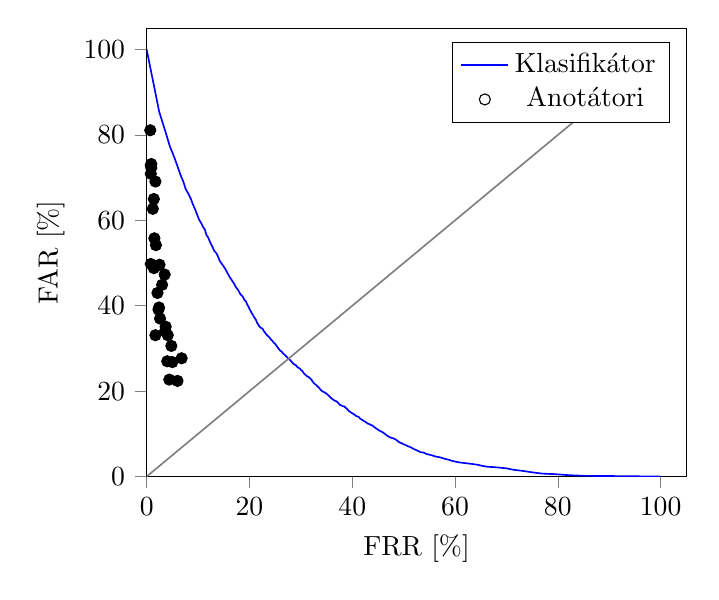
\begin{tikzpicture}

\begin{axis}[
tick align=outside,
tick pos=left,
x grid style={white!69.01960784313725!black},
xlabel={FRR [\%]},
xmin=0, xmax=105,
y grid style={white!69.01960784313725!black},
ylabel={FAR [\%]},
ymin=0, ymax=105,
legend pos=north east,
]

\addplot [semithick, blue]
table {%
0 100
2.43801807884175 85.4384553499598
3.64202393008514 80.8125502815768
4.51220884437943 77.3129525341915
5.31112861483065 74.9798873692679
5.96001650350699 72.8077232502011
6.55639323356213 70.7160096540627
7.10776039908481 69.147224456959
7.58786242076441 67.33708769107
8.09046922471025 66.2912308930008
8.55556805821237 65.1649235720032
8.94190015378268 63.917940466613
9.38074340797419 62.711182622687
9.79708187989948 61.4239742558327
10.1871647725142 60.1769911504425
10.6035032444394 59.3724859211585
10.9335733843442 58.5277554304103
11.334908668092 57.8037007240547
11.6387232286861 56.5567176186645
11.9537901804133 55.9935639581657
12.2951127114512 55.0281576830249
12.5614193016016 54.3443282381335
12.8914894415063 53.5398230088496
13.1878024080117 52.7755430410298
13.5703837065376 52.3330651649236
13.9117062375755 51.407884151247
14.2117700011252 50.5229283990346
14.5530925321631 49.9195494770716
14.8494054986685 49.4368463395012
15.1344660740407 48.9139179404666
15.4457822287236 48.3105390185036
15.7158396159184 47.6669348350764
15.9821462060688 47.1037811745776
16.2672067814411 46.5004022526146
16.5147593863696 46.0981496379726
16.7548103972094 45.6154465004022
16.9798582198717 45.2534191472245
17.234912418889 44.6098149637973
17.5199729942613 44.0868865647627
17.8050335696335 43.6846339501207
18.0263305952515 43.1617055510861
18.2701324031357 42.6387771520515
18.5476913844192 42.3572003218021
18.8064963804809 41.8744971842317
19.0390457972319 41.3113435237329
19.3241063726042 40.9895414320193
19.5379018041334 40.3459372485921
19.8079591913282 39.7827835880933
20.0330070139905 39.1794046661303
20.1905404898541 38.8576025744167
20.4043359213833 38.3748994368463
20.603128164735 38.0128720836685
20.7869172199092 37.5703942075623
21.026968230749 37.1279163314562
21.248265256367 36.7256637168142
21.5145718465174 35.9613837489944
21.7283672780466 35.5591311343524
21.9196579273096 35.1971037811746
22.1109485765725 34.9155269509252
22.347248790368 34.7546259050684
22.5572934248528 34.5937248592116
22.7898428416038 34.070796460177
22.9886350849556 33.7892196299276
23.2211845017066 33.3869670152856
23.4799894977683 33.0249396621078
23.7125389145193 32.7835880933226
23.9263343460485 32.5422365245374
24.1963917332433 32.059533386967
24.4777015115712 31.7779565567176
24.7290049135441 31.3354786806114
24.9953115036945 31.0941271118262
25.2241101234012 30.6918744971842
25.4416563519748 30.3298471440064
25.6141930160159 30.048270313757
25.8354900416338 29.6862429605792
26.008026705675 29.444891391794
26.2518285135591 29.2839903459372
26.4656239450883 28.9219629927595
26.7131765500169 28.6403861625101
26.9082179963242 28.4392598551891
27.1707737894303 28.1174577634755
27.3808184239151 27.8761061946903
27.6171186377105 27.5140788415125
27.8796744308165 27.3129525341915
28.085968268257 27.0313757039421
28.27725891752 26.7900241351569
28.4873035520048 26.4682220434433
28.7048497805784 26.2670957361223
28.9298976032407 26.1866452131939
29.1024342672818 25.9855189058729
29.3649900603878 25.5832662912309
29.5675331007839 25.4625905068383
29.83008889389 25.2614641995173
30.0401335283748 24.9396621078037
30.2764337421702 24.7385358004827
30.4752259855219 24.3765084473049
30.7227785904505 23.9742558326629
30.9328232249353 23.8133547868061
31.2103822062188 23.4513274336283
31.4616856081917 23.3708769106999
31.716739807209 23.0893000804505
31.908030456472 22.8881737731295
32.1105734968681 22.6065969428801
32.2981133490867 22.2445695897023
32.523161171749 21.8825422365245
32.7632121825888 21.6009654062751
33.0107647875174 21.4400643604183
33.2245602190465 21.1182622687047
33.5021192003301 20.8366854384553
33.7384194141255 20.4746580852776
33.9972244101872 20.1126307320998
34.2260230298939 19.951729686243
34.4773264318668 19.7908286403862
34.6873710663516 19.6701528559936
34.9011664978808 19.4690265486726
35.1674730880312 19.2276749798874
35.467536851581 18.9058728881738
35.7450958328645 18.543845534996
36.0076516259705 18.2622687047466
36.2814598102097 18.0209171359614
36.5552679944488 17.7795655671762
36.7878174111999 17.6991150442478
37.1066351599715 17.4577634754626
37.3541877649 17.135961383749
37.6429991373167 16.733708769107
37.898053336334 16.6532582461786
38.1231011589963 16.4923572003218
38.4606728929898 16.4119066773934
38.7269794831402 16.0901045856798
39.0120400585124 15.8085277554304
39.2708450545741 15.4062751407884
39.5634072240351 15.1649235720032
39.8522185964517 14.923572003218
40.2010427215783 14.6822204344328
40.4485953265069 14.4810941271118
40.6848955403023 14.2397425583266
40.973706912719 14.0788415124698
41.2700198792243 13.9581657280772
41.5663328457297 13.515687851971
41.8889013915457 13.31456154465
42.1589587787405 13.0732099758648
42.4590225422902 12.8720836685438
42.7740894940175 12.6307320997586
43.0178913019017 12.3893805309735
43.2916994861408 12.3089300080451
43.6142680319568 12.0675784392599
43.9068302014178 11.9871279163315
44.1918907767901 11.6653258246179
44.5182101196504 11.3837489943685
44.8632834477326 11.1021721641191
45.2421139492142 10.7803700724055
45.613442856607 10.5792437650845
45.9097558231124 10.3781174577635
46.2473275571059 10.0965406275141
46.6561644349424 9.69428801287208
47.0537489216458 9.37248592115849
47.4325794231274 9.13113435237329
47.9051798507183 8.97023330651649
48.3327707137767 8.7691069991955
48.749109185702 8.4070796460177
49.1616968605829 8.0048270313757
49.5555305502419 7.84392598551891
49.9718690221672 7.56234915526951
50.433217058625 7.36122284794851
50.887063500994 7.07964601769912
51.3446607404073 6.87851971037812
51.8060087768651 6.55671761866452
52.2936123926334 6.27514078841512
52.833727167023 5.99356395816573
53.3738419414126 5.67176186645213
53.8764487453584 5.63153660498793
54.386557143393 5.30973451327434
54.9041671355163 5.14883346741754
55.4930422714827 4.98793242156074
56.141930160159 4.70635559131134
56.6895465286373 4.58567980691874
57.3159296350474 4.42477876106195
58.0248302764337 4.14320193081255
58.7524849030419 3.94207562349155
59.4801395296501 3.66049879324216
60.1965417651251 3.45937248592116
60.9091932035558 3.29847144006436
61.7043621769626 3.17779565567176
62.5820486853456 3.05711987127916
63.3659652676194 2.93644408688656
64.3186677168898 2.77554304102977
65.3351337159146 2.49396621078037
66.2878361651851 2.29283990345937
67.4430816548517 2.21238938053097
68.6208319267844 2.09171359613838
69.9523648775365 1.93081255028158
71.4639360864184 1.56878519710378
73.1630471475188 1.32743362831858
74.8921645849743 1.00563153660499
77.0226173061776 0.683829444891392
79.3443606766438 0.563153660498793
82.1161996924346 0.321802091713596
85.4169010914819 0.160901045856798
89.9966242826601 0.120675784392599
100 0
};
\addlegendentry{Klasifikátor}

\addplot [scatter, only marks, scatter src=explicit symbolic,
          scatter/classes={
            a={mark=o, draw=black, fill=black}
          }
]
table {%
3.50 31.2 a 
3.60 34.1 a 
0.80 49.8 a 
6.00 22.4 a 
3.50 47.3 a 
1.20 62.7 a 
2.30 39.1 a 
0.90 73.2 a 
4.80 30.6 a 
2.50 49.6 a 
1.40 65.0 a 
2.40 39.6 a 
0.80 70.9 a 
4.40 22.7 a 
2.10 43.0 a 
1.70 33.1 a 
4.10 33.1 a 
4.00 27.0 a 
6.80 27.7 a 
3.70 35.1 a 
0.80 72.9 a 
1.80 54.2 a 
1.40 48.8 a 
0.70 81.1 a 
1.50 55.8 a 
1.70 69.1 a 
3.00 44.9 a 
2.60 37.0 a 
0.90 72.3 a 
5.00 26.8 a
}; \addlegendentry{Anotátori}

\addplot [semithick, gray, forget plot]
table [row sep=\\]{%
0	0 \\
0.50251256281407	0.50251256281407 \\
1.00502512562814	1.00502512562814 \\
1.50753768844221	1.50753768844221 \\
2.01005025125628	2.01005025125628 \\
2.51256281407035	2.51256281407035 \\
3.01507537688442	3.01507537688442 \\
3.51758793969849	3.51758793969849 \\
4.02010050251256	4.02010050251256 \\
4.52261306532663	4.52261306532663 \\
5.0251256281407	5.0251256281407 \\
5.52763819095477	5.52763819095477 \\
6.03015075376884	6.03015075376884 \\
6.53266331658291	6.53266331658291 \\
7.03517587939698	7.03517587939698 \\
7.53768844221105	7.53768844221105 \\
8.04020100502512	8.04020100502512 \\
8.5427135678392	8.5427135678392 \\
9.04522613065327	9.04522613065327 \\
9.54773869346734	9.54773869346734 \\
10.0502512562814	10.0502512562814 \\
10.5527638190955	10.5527638190955 \\
11.0552763819095	11.0552763819095 \\
11.5577889447236	11.5577889447236 \\
12.0603015075377	12.0603015075377 \\
12.5628140703518	12.5628140703518 \\
13.0653266331658	13.0653266331658 \\
13.5678391959799	13.5678391959799 \\
14.070351758794	14.070351758794 \\
14.572864321608	14.572864321608 \\
15.0753768844221	15.0753768844221 \\
15.5778894472362	15.5778894472362 \\
16.0804020100502	16.0804020100502 \\
16.5829145728643	16.5829145728643 \\
17.0854271356784	17.0854271356784 \\
17.5879396984925	17.5879396984925 \\
18.0904522613065	18.0904522613065 \\
18.5929648241206	18.5929648241206 \\
19.0954773869347	19.0954773869347 \\
19.5979899497487	19.5979899497487 \\
20.1005025125628	20.1005025125628 \\
20.6030150753769	20.6030150753769 \\
21.105527638191	21.105527638191 \\
21.608040201005	21.608040201005 \\
22.1105527638191	22.1105527638191 \\
22.6130653266332	22.6130653266332 \\
23.1155778894472	23.1155778894472 \\
23.6180904522613	23.6180904522613 \\
24.1206030150754	24.1206030150754 \\
24.6231155778894	24.6231155778894 \\
25.1256281407035	25.1256281407035 \\
25.6281407035176	25.6281407035176 \\
26.1306532663317	26.1306532663317 \\
26.6331658291457	26.6331658291457 \\
27.1356783919598	27.1356783919598 \\
27.6381909547739	27.6381909547739 \\
28.1407035175879	28.1407035175879 \\
28.643216080402	28.643216080402 \\
29.1457286432161	29.1457286432161 \\
29.6482412060301	29.6482412060301 \\
30.1507537688442	30.1507537688442 \\
30.6532663316583	30.6532663316583 \\
31.1557788944724	31.1557788944724 \\
31.6582914572864	31.6582914572864 \\
32.1608040201005	32.1608040201005 \\
32.6633165829146	32.6633165829146 \\
33.1658291457286	33.1658291457286 \\
33.6683417085427	33.6683417085427 \\
34.1708542713568	34.1708542713568 \\
34.6733668341708	34.6733668341708 \\
35.1758793969849	35.1758793969849 \\
35.678391959799	35.678391959799 \\
36.1809045226131	36.1809045226131 \\
36.6834170854271	36.6834170854271 \\
37.1859296482412	37.1859296482412 \\
37.6884422110553	37.6884422110553 \\
38.1909547738693	38.1909547738693 \\
38.6934673366834	38.6934673366834 \\
39.1959798994975	39.1959798994975 \\
39.6984924623116	39.6984924623116 \\
40.2010050251256	40.2010050251256 \\
40.7035175879397	40.7035175879397 \\
41.2060301507538	41.2060301507538 \\
41.7085427135678	41.7085427135678 \\
42.2110552763819	42.2110552763819 \\
42.713567839196	42.713567839196 \\
43.21608040201	43.21608040201 \\
43.7185929648241	43.7185929648241 \\
44.2211055276382	44.2211055276382 \\
44.7236180904523	44.7236180904523 \\
45.2261306532663	45.2261306532663 \\
45.7286432160804	45.7286432160804 \\
46.2311557788945	46.2311557788945 \\
46.7336683417085	46.7336683417085 \\
47.2361809045226	47.2361809045226 \\
47.7386934673367	47.7386934673367 \\
48.2412060301507	48.2412060301507 \\
48.7437185929648	48.7437185929648 \\
49.2462311557789	49.2462311557789 \\
49.748743718593	49.748743718593 \\
50.251256281407	50.251256281407 \\
50.7537688442211	50.7537688442211 \\
51.2562814070352	51.2562814070352 \\
51.7587939698492	51.7587939698492 \\
52.2613065326633	52.2613065326633 \\
52.7638190954774	52.7638190954774 \\
53.2663316582914	53.2663316582914 \\
53.7688442211055	53.7688442211055 \\
54.2713567839196	54.2713567839196 \\
54.7738693467337	54.7738693467337 \\
55.2763819095477	55.2763819095477 \\
55.7788944723618	55.7788944723618 \\
56.2814070351759	56.2814070351759 \\
56.7839195979899	56.7839195979899 \\
57.286432160804	57.286432160804 \\
57.7889447236181	57.7889447236181 \\
58.2914572864322	58.2914572864322 \\
58.7939698492462	58.7939698492462 \\
59.2964824120603	59.2964824120603 \\
59.7989949748744	59.7989949748744 \\
60.3015075376884	60.3015075376884 \\
60.8040201005025	60.8040201005025 \\
61.3065326633166	61.3065326633166 \\
61.8090452261306	61.8090452261306 \\
62.3115577889447	62.3115577889447 \\
62.8140703517588	62.8140703517588 \\
63.3165829145729	63.3165829145729 \\
63.8190954773869	63.8190954773869 \\
64.321608040201	64.321608040201 \\
64.8241206030151	64.8241206030151 \\
65.3266331658291	65.3266331658291 \\
65.8291457286432	65.8291457286432 \\
66.3316582914573	66.3316582914573 \\
66.8341708542713	66.8341708542713 \\
67.3366834170854	67.3366834170854 \\
67.8391959798995	67.8391959798995 \\
68.3417085427136	68.3417085427136 \\
68.8442211055276	68.8442211055276 \\
69.3467336683417	69.3467336683417 \\
69.8492462311558	69.8492462311558 \\
70.3517587939699	70.3517587939699 \\
70.8542713567839	70.8542713567839 \\
71.356783919598	71.356783919598 \\
71.859296482412	71.859296482412 \\
72.3618090452261	72.3618090452261 \\
72.8643216080402	72.8643216080402 \\
73.3668341708543	73.3668341708543 \\
73.8693467336683	73.8693467336683 \\
74.3718592964824	74.3718592964824 \\
74.8743718592965	74.8743718592965 \\
75.3768844221105	75.3768844221105 \\
75.8793969849246	75.8793969849246 \\
76.3819095477387	76.3819095477387 \\
76.8844221105528	76.8844221105528 \\
77.3869346733668	77.3869346733668 \\
77.8894472361809	77.8894472361809 \\
78.391959798995	78.391959798995 \\
78.894472361809	78.894472361809 \\
79.3969849246231	79.3969849246231 \\
79.8994974874372	79.8994974874372 \\
80.4020100502512	80.4020100502512 \\
80.9045226130653	80.9045226130653 \\
81.4070351758794	81.4070351758794 \\
81.9095477386935	81.9095477386935 \\
82.4120603015075	82.4120603015075 \\
82.9145728643216	82.9145728643216 \\
83.4170854271357	83.4170854271357 \\
83.9195979899497	83.9195979899497 \\
84.4221105527638	84.4221105527638 \\
84.9246231155779	84.9246231155779 \\
85.4271356783919	85.4271356783919 \\
85.929648241206	85.929648241206 \\
86.4321608040201	86.4321608040201 \\
86.9346733668342	86.9346733668342 \\
87.4371859296482	87.4371859296482 \\
87.9396984924623	87.9396984924623 \\
88.4422110552764	88.4422110552764 \\
88.9447236180904	88.9447236180904 \\
89.4472361809045	89.4472361809045 \\
89.9497487437186	89.9497487437186 \\
90.4522613065326	90.4522613065326 \\
90.9547738693467	90.9547738693467 \\
91.4572864321608	91.4572864321608 \\
91.9597989949749	91.9597989949749 \\
92.4623115577889	92.4623115577889 \\
92.964824120603	92.964824120603 \\
93.4673366834171	93.4673366834171 \\
93.9698492462311	93.9698492462311 \\
94.4723618090452	94.4723618090452 \\
94.9748743718593	94.9748743718593 \\
95.4773869346734	95.4773869346734 \\
95.9798994974874	95.9798994974874 \\
96.4824120603015	96.4824120603015 \\
96.9849246231156	96.9849246231156 \\
97.4874371859296	97.4874371859296 \\
97.9899497487437	97.9899497487437 \\
98.4924623115578	98.4924623115578 \\
98.9949748743718	98.9949748743718 \\
99.4974874371859	99.4974874371859 \\
100	100 \\
};

\end{axis}

\end{tikzpicture}}
    \caption{Všetky fonémy}
\end{subfigure}
\begin{subfigure}[b]{0.49\textwidth}
    \resizebox{\textwidth}{!}{% This file was created by matplotlib2tikz v0.6.18.
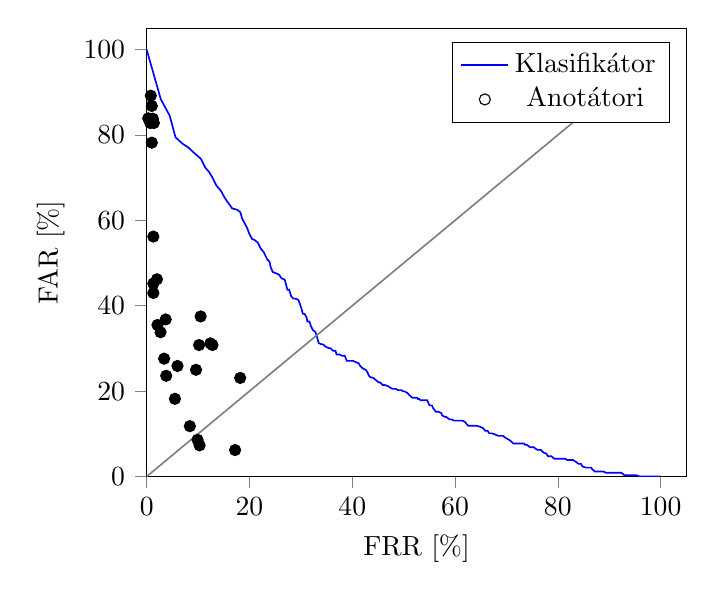
\begin{tikzpicture}

\begin{axis}[
tick align=outside,
tick pos=left,
x grid style={white!69.01960784313725!black},
xlabel={FRR [\%]},
xmin=0, xmax=105,
y grid style={white!69.01960784313725!black},
ylabel={FAR [\%]},
ymin=0, ymax=105,
legend pos=north east,
]

\addplot [semithick, blue]
table {%
0 100
2.73881095524382 88.3928571428571
4.47561790247161 84.5238095238095
5.61122244488978 79.4642857142857
6.94722778891116 77.9761904761905
8.08283233132933 77.0833333333333
9.15163660654643 75.8928571428571
10.5544422177689 74.4047619047619
11.4228456913828 72.3214285714286
12.0908483633935 71.4285714285714
12.6920507682031 70.2380952380952
13.560454241817 68.1547619047619
14.4288577154309 66.9642857142857
15.0968603874415 65.4761904761905
15.564462257849 64.5833333333333
16.2992651970608 63.3928571428571
16.6332665330661 62.797619047619
17.5684702738811 62.5
18.2364729458918 61.9047619047619
18.5704742818971 60.4166666666667
19.1048764195057 59.2261904761905
19.5056780227121 58.3333333333333
19.9732798931196 56.8452380952381
20.5076820307281 55.6547619047619
21.0420841683367 55.3571428571429
21.6432865731463 54.7619047619048
22.2444889779559 53.2738095238095
22.7120908483634 52.6785714285714
23.4468937875752 50.8928571428571
23.9144956579826 50.297619047619
24.1148964595858 49.1071428571429
24.315297261189 48.5119047619048
24.5156980627923 47.9166666666667
25.1169004676019 47.6190476190476
25.7181028724115 47.3214285714286
26.25250501002 46.4285714285714
26.8537074148297 46.1309523809524
27.0541082164329 45.2380952380952
27.3881095524382 43.75
27.7221108884436 43.75
28.12291249165 42.2619047619048
28.5237140948564 41.6666666666667
28.9245156980628 41.6666666666667
29.5257181028724 41.3690476190476
30.060120240481 39.5833333333333
30.2605210420842 38.6904761904762
30.3941215764863 38.0952380952381
30.7281229124916 38.0952380952381
31.1289245156981 37.202380952381
31.2625250501002 36.3095238095238
31.6633266533066 36.3095238095238
31.997327989312 35.1190476190476
32.3981295925184 34.2261904761905
32.7989311957248 33.9285714285714
33.0661322645291 33.0357142857143
33.4669338677355 31.25
34.0681362725451 30.952380952381
34.3353373413494 30.952380952381
34.8697394789579 30.3571428571429
35.5377421509686 30.0595238095238
35.7381429525718 30.0595238095238
36.2725450901804 29.4642857142857
36.7401469605878 29.4642857142857
36.9405477621911 28.5714285714286
37.5417501670007 28.5714285714286
38.0093520374081 28.2738095238095
38.5437541750167 28.2738095238095
38.9445557782231 27.0833333333333
39.6125584502338 27.0833333333333
40.1469605878424 27.0833333333333
40.748162992652 26.7857142857143
41.2825651302605 26.4880952380952
41.5497661990648 25.8928571428571
41.8169672678691 25.5952380952381
42.0841683366733 25.297619047619
42.6185704742819 25
42.9525718102872 24.4047619047619
43.2865731462926 23.5119047619048
43.6205744822979 23.2142857142857
43.8877755511022 23.2142857142857
44.2885771543086 22.9166666666667
44.5557782231129 22.6190476190476
45.2237808951236 22.0238095238095
45.4909819639279 22.0238095238095
45.8917835671343 21.4285714285714
46.3593854375418 21.4285714285714
47.0273881095524 21.1309523809524
47.3613894455578 20.8333333333333
47.8289913159653 20.5357142857143
48.4969939879759 20.5357142857143
48.8977955911824 20.2380952380952
49.2317969271877 20.2380952380952
49.5657982631931 20.2380952380952
49.8997995991984 19.9404761904762
50.2338009352037 19.9404761904762
50.5678022712091 19.6428571428571
50.7014028056112 19.6428571428571
51.1022044088176 19.047619047619
51.7034068136273 18.452380952381
51.8370073480294 18.452380952381
52.2378089512358 18.452380952381
52.6386105544422 18.452380952381
52.7722110888444 18.1547619047619
53.0394121576486 18.1547619047619
53.3066132264529 17.8571428571429
54.1082164328657 17.8571428571429
54.5758183032732 17.8571428571429
55.0434201736807 16.6666666666667
55.5110220440882 16.6666666666667
55.7114228456914 16.0714285714286
56.2458249832999 15.1785714285714
56.7134268537074 15.1785714285714
57.314629258517 14.8809523809524
57.5150300601202 14.2857142857143
57.9826319305277 13.9880952380952
58.249832999332 13.9880952380952
58.9178356713427 13.3928571428571
59.3186372745491 13.3928571428571
59.7862391449566 13.0952380952381
60.7214428857716 13.0952380952381
61.0554442217769 13.0952380952381
61.4562458249833 13.0952380952381
61.9238476953908 12.797619047619
62.3246492985972 12.202380952381
62.5918503674015 11.9047619047619
62.9258517034068 11.9047619047619
63.3266533066132 11.9047619047619
64.1950567802271 11.9047619047619
64.99665998664 11.6071428571429
65.4642618570474 11.3095238095238
65.8650634602538 10.7142857142857
66.3326653306613 10.7142857142857
66.6666666666667 10.1190476190476
67.2010688042752 10.1190476190476
67.8690714762859 9.82142857142857
68.4034736138945 9.52380952380952
68.6038744154977 9.52380952380952
69.4054776219105 9.52380952380952
69.6058784235137 9.22619047619048
70.0066800267201 8.92857142857143
70.4742818971276 8.63095238095238
70.8082832331329 8.33333333333333
71.3426853707415 7.73809523809524
71.7434869739479 7.73809523809524
72.0774883099532 7.73809523809524
72.4782899131597 7.73809523809524
72.9458917835671 7.73809523809524
73.4134936539746 7.73809523809524
73.6138944555778 7.44047619047619
73.9478957915832 7.44047619047619
74.6158984635939 6.8452380952381
75.3507014028056 6.8452380952381
75.6179024716099 6.54761904761905
76.0187040748163 6.25
76.686706746827 6.25
77.1543086172345 5.65476190476191
77.7555110220441 5.35714285714286
78.0895123580494 4.76190476190476
78.2899131596526 4.76190476190476
78.7575150300601 4.76190476190476
79.2919171676687 4.16666666666667
79.4923179692719 4.16666666666667
79.8931195724783 4.16666666666667
80.7615230460922 4.16666666666667
81.4295257181029 4.16666666666667
81.8303273213093 3.86904761904762
82.3647294589178 3.86904761904762
82.9659318637275 3.86904761904762
83.7007348029392 3.27380952380952
84.0347361389446 2.97619047619048
84.502338009352 2.97619047619048
84.7695390781563 2.38095238095238
85.437541750167 2.08333333333333
85.8383433533734 2.08333333333333
86.5063460253841 2.08333333333333
86.6399465597862 1.78571428571429
87.1743486973948 1.19047619047619
87.6419505678023 1.19047619047619
88.1763527054108 1.19047619047619
88.8443553774215 1.19047619047619
89.3787575150301 0.892857142857143
89.9799599198397 0.892857142857143
90.4475617902472 0.892857142857143
91.0487641950568 0.892857142857143
91.7167668670675 0.892857142857143
92.3847695390782 0.892857142857143
92.6519706078824 0.595238095238095
92.9859719438878 0.297619047619048
93.3199732798931 0.297619047619048
93.9879759519038 0.297619047619048
94.5891783567134 0.297619047619048
95.2571810287241 0.297619047619048
95.9251837007348 0
96.5931863727455 0
97.127588510354 0
97.6619906479626 0
98.1295925183701 0
98.997995991984 0
99.2651970607882 0
100 0
};
\addlegendentry{Klasifikátor}

\addplot [scatter, only marks, scatter src=explicit symbolic,
          scatter/classes={
            a={mark=o, draw=black, fill=black}
          }
]
table {%
10.4 23.1 a
10.2 30.8 a
02.0 46.2 a
12.8 30.8 a
18.2 23.1 a
00.7 82.8 a
03.4 27.6 a
01.4 82.8 a
06.0 25.9 a
09.9 08.6 a
01.0 83.6 a
03.8 23.6 a
01.0 78.2 a
05.5 18.2 a
10.3 07.3 a
01.3 56.2 a
10.5 37.5 a
09.6 25.0 a
12.4 31.2 a
17.2 06.2 a
01.0 86.8 a
03.7 36.8 a
02.7 33.8 a
01.2 83.8 a
08.4 11.8 a
00.8 89.2 a
01.3 43.0 a
01.3 45.2 a
00.3 83.9 a
02.1 35.5 a
}; \addlegendentry{Anotátori}


\addplot [semithick, gray, forget plot]
table [row sep=\\]{%
0	0 \\
0.50251256281407	0.50251256281407 \\
1.00502512562814	1.00502512562814 \\
1.50753768844221	1.50753768844221 \\
2.01005025125628	2.01005025125628 \\
2.51256281407035	2.51256281407035 \\
3.01507537688442	3.01507537688442 \\
3.51758793969849	3.51758793969849 \\
4.02010050251256	4.02010050251256 \\
4.52261306532663	4.52261306532663 \\
5.0251256281407	5.0251256281407 \\
5.52763819095477	5.52763819095477 \\
6.03015075376884	6.03015075376884 \\
6.53266331658291	6.53266331658291 \\
7.03517587939698	7.03517587939698 \\
7.53768844221105	7.53768844221105 \\
8.04020100502512	8.04020100502512 \\
8.5427135678392	8.5427135678392 \\
9.04522613065327	9.04522613065327 \\
9.54773869346734	9.54773869346734 \\
10.0502512562814	10.0502512562814 \\
10.5527638190955	10.5527638190955 \\
11.0552763819095	11.0552763819095 \\
11.5577889447236	11.5577889447236 \\
12.0603015075377	12.0603015075377 \\
12.5628140703518	12.5628140703518 \\
13.0653266331658	13.0653266331658 \\
13.5678391959799	13.5678391959799 \\
14.070351758794	14.070351758794 \\
14.572864321608	14.572864321608 \\
15.0753768844221	15.0753768844221 \\
15.5778894472362	15.5778894472362 \\
16.0804020100502	16.0804020100502 \\
16.5829145728643	16.5829145728643 \\
17.0854271356784	17.0854271356784 \\
17.5879396984925	17.5879396984925 \\
18.0904522613065	18.0904522613065 \\
18.5929648241206	18.5929648241206 \\
19.0954773869347	19.0954773869347 \\
19.5979899497487	19.5979899497487 \\
20.1005025125628	20.1005025125628 \\
20.6030150753769	20.6030150753769 \\
21.105527638191	21.105527638191 \\
21.608040201005	21.608040201005 \\
22.1105527638191	22.1105527638191 \\
22.6130653266332	22.6130653266332 \\
23.1155778894472	23.1155778894472 \\
23.6180904522613	23.6180904522613 \\
24.1206030150754	24.1206030150754 \\
24.6231155778894	24.6231155778894 \\
25.1256281407035	25.1256281407035 \\
25.6281407035176	25.6281407035176 \\
26.1306532663317	26.1306532663317 \\
26.6331658291457	26.6331658291457 \\
27.1356783919598	27.1356783919598 \\
27.6381909547739	27.6381909547739 \\
28.1407035175879	28.1407035175879 \\
28.643216080402	28.643216080402 \\
29.1457286432161	29.1457286432161 \\
29.6482412060301	29.6482412060301 \\
30.1507537688442	30.1507537688442 \\
30.6532663316583	30.6532663316583 \\
31.1557788944724	31.1557788944724 \\
31.6582914572864	31.6582914572864 \\
32.1608040201005	32.1608040201005 \\
32.6633165829146	32.6633165829146 \\
33.1658291457286	33.1658291457286 \\
33.6683417085427	33.6683417085427 \\
34.1708542713568	34.1708542713568 \\
34.6733668341708	34.6733668341708 \\
35.1758793969849	35.1758793969849 \\
35.678391959799	35.678391959799 \\
36.1809045226131	36.1809045226131 \\
36.6834170854271	36.6834170854271 \\
37.1859296482412	37.1859296482412 \\
37.6884422110553	37.6884422110553 \\
38.1909547738693	38.1909547738693 \\
38.6934673366834	38.6934673366834 \\
39.1959798994975	39.1959798994975 \\
39.6984924623116	39.6984924623116 \\
40.2010050251256	40.2010050251256 \\
40.7035175879397	40.7035175879397 \\
41.2060301507538	41.2060301507538 \\
41.7085427135678	41.7085427135678 \\
42.2110552763819	42.2110552763819 \\
42.713567839196	42.713567839196 \\
43.21608040201	43.21608040201 \\
43.7185929648241	43.7185929648241 \\
44.2211055276382	44.2211055276382 \\
44.7236180904523	44.7236180904523 \\
45.2261306532663	45.2261306532663 \\
45.7286432160804	45.7286432160804 \\
46.2311557788945	46.2311557788945 \\
46.7336683417085	46.7336683417085 \\
47.2361809045226	47.2361809045226 \\
47.7386934673367	47.7386934673367 \\
48.2412060301507	48.2412060301507 \\
48.7437185929648	48.7437185929648 \\
49.2462311557789	49.2462311557789 \\
49.748743718593	49.748743718593 \\
50.251256281407	50.251256281407 \\
50.7537688442211	50.7537688442211 \\
51.2562814070352	51.2562814070352 \\
51.7587939698492	51.7587939698492 \\
52.2613065326633	52.2613065326633 \\
52.7638190954774	52.7638190954774 \\
53.2663316582914	53.2663316582914 \\
53.7688442211055	53.7688442211055 \\
54.2713567839196	54.2713567839196 \\
54.7738693467337	54.7738693467337 \\
55.2763819095477	55.2763819095477 \\
55.7788944723618	55.7788944723618 \\
56.2814070351759	56.2814070351759 \\
56.7839195979899	56.7839195979899 \\
57.286432160804	57.286432160804 \\
57.7889447236181	57.7889447236181 \\
58.2914572864322	58.2914572864322 \\
58.7939698492462	58.7939698492462 \\
59.2964824120603	59.2964824120603 \\
59.7989949748744	59.7989949748744 \\
60.3015075376884	60.3015075376884 \\
60.8040201005025	60.8040201005025 \\
61.3065326633166	61.3065326633166 \\
61.8090452261306	61.8090452261306 \\
62.3115577889447	62.3115577889447 \\
62.8140703517588	62.8140703517588 \\
63.3165829145729	63.3165829145729 \\
63.8190954773869	63.8190954773869 \\
64.321608040201	64.321608040201 \\
64.8241206030151	64.8241206030151 \\
65.3266331658291	65.3266331658291 \\
65.8291457286432	65.8291457286432 \\
66.3316582914573	66.3316582914573 \\
66.8341708542713	66.8341708542713 \\
67.3366834170854	67.3366834170854 \\
67.8391959798995	67.8391959798995 \\
68.3417085427136	68.3417085427136 \\
68.8442211055276	68.8442211055276 \\
69.3467336683417	69.3467336683417 \\
69.8492462311558	69.8492462311558 \\
70.3517587939699	70.3517587939699 \\
70.8542713567839	70.8542713567839 \\
71.356783919598	71.356783919598 \\
71.859296482412	71.859296482412 \\
72.3618090452261	72.3618090452261 \\
72.8643216080402	72.8643216080402 \\
73.3668341708543	73.3668341708543 \\
73.8693467336683	73.8693467336683 \\
74.3718592964824	74.3718592964824 \\
74.8743718592965	74.8743718592965 \\
75.3768844221105	75.3768844221105 \\
75.8793969849246	75.8793969849246 \\
76.3819095477387	76.3819095477387 \\
76.8844221105528	76.8844221105528 \\
77.3869346733668	77.3869346733668 \\
77.8894472361809	77.8894472361809 \\
78.391959798995	78.391959798995 \\
78.894472361809	78.894472361809 \\
79.3969849246231	79.3969849246231 \\
79.8994974874372	79.8994974874372 \\
80.4020100502512	80.4020100502512 \\
80.9045226130653	80.9045226130653 \\
81.4070351758794	81.4070351758794 \\
81.9095477386935	81.9095477386935 \\
82.4120603015075	82.4120603015075 \\
82.9145728643216	82.9145728643216 \\
83.4170854271357	83.4170854271357 \\
83.9195979899497	83.9195979899497 \\
84.4221105527638	84.4221105527638 \\
84.9246231155779	84.9246231155779 \\
85.4271356783919	85.4271356783919 \\
85.929648241206	85.929648241206 \\
86.4321608040201	86.4321608040201 \\
86.9346733668342	86.9346733668342 \\
87.4371859296482	87.4371859296482 \\
87.9396984924623	87.9396984924623 \\
88.4422110552764	88.4422110552764 \\
88.9447236180904	88.9447236180904 \\
89.4472361809045	89.4472361809045 \\
89.9497487437186	89.9497487437186 \\
90.4522613065326	90.4522613065326 \\
90.9547738693467	90.9547738693467 \\
91.4572864321608	91.4572864321608 \\
91.9597989949749	91.9597989949749 \\
92.4623115577889	92.4623115577889 \\
92.964824120603	92.964824120603 \\
93.4673366834171	93.4673366834171 \\
93.9698492462311	93.9698492462311 \\
94.4723618090452	94.4723618090452 \\
94.9748743718593	94.9748743718593 \\
95.4773869346734	95.4773869346734 \\
95.9798994974874	95.9798994974874 \\
96.4824120603015	96.4824120603015 \\
96.9849246231156	96.9849246231156 \\
97.4874371859296	97.4874371859296 \\
97.9899497487437	97.9899497487437 \\
98.4924623115578	98.4924623115578 \\
98.9949748743718	98.9949748743718 \\
99.4974874371859	99.4974874371859 \\
100	100 \\
};

\end{axis}

\end{tikzpicture}}
    \caption{Fonéma \textipa{/@/}}
\end{subfigure}
\par\vspace{2em}
\begin{subfigure}[b]{0.49\textwidth}
    \resizebox{\textwidth}{!}{% This file was created by matplotlib2tikz v0.6.18.
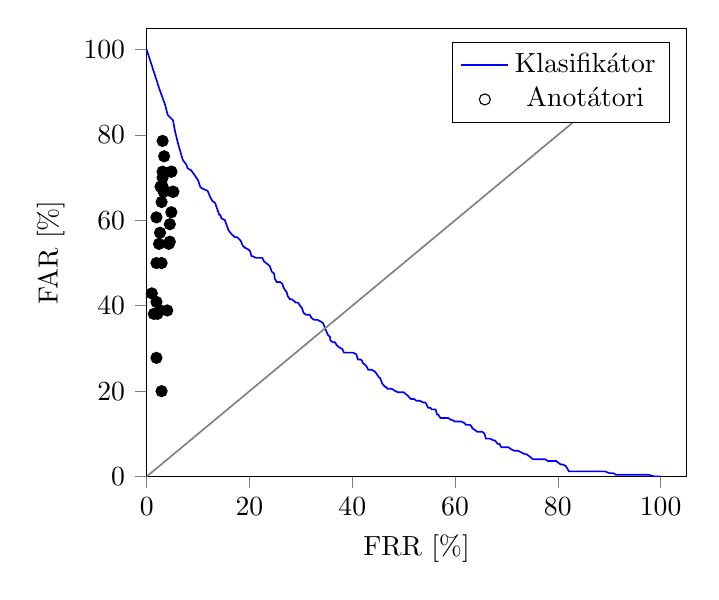
\begin{tikzpicture}

\begin{axis}[
tick align=outside,
tick pos=left,
x grid style={white!69.01960784313725!black},
xlabel={FRR [\%]},
xmin=0, xmax=105,
y grid style={white!69.01960784313725!black},
ylabel={FAR [\%]},
ymin=0, ymax=105,
legend pos=north east,
]

\addplot [semithick, blue]
table {%
0 100
2.48538011695906 90.7258064516129
3.58187134502924 87.0967741935484
4.09356725146199 84.6774193548387
5.11695906432749 83.4677419354839
5.55555555555556 80.6451612903226
6.14035087719298 77.8225806451613
7.01754385964912 74.1935483870968
7.74853801169591 72.9838709677419
7.96783625730994 72.1774193548387
8.62573099415205 71.7741935483871
9.57602339181287 70.1612903225807
10.0146198830409 69.3548387096774
10.453216374269 67.741935483871
11.0380116959064 67.3387096774193
11.8421052631579 66.9354838709677
12.280701754386 65.7258064516129
12.4269005847953 65.3225806451613
12.7923976608187 64.5161290322581
13.3040935672515 64.1129032258064
13.8888888888889 62.0967741935484
14.1081871345029 61.2903225806452
14.327485380117 61.2903225806452
14.546783625731 60.4838709677419
15.2046783625731 60.0806451612903
15.9356725146199 57.6612903225806
16.4473684210526 56.8548387096774
16.812865497076 56.4516129032258
17.1783625730994 56.0483870967742
17.6169590643275 56.0483870967742
18.2748538011696 55.241935483871
18.7134502923977 54.0322580645161
19.0789473684211 53.6290322580645
19.7368421052632 53.2258064516129
20.1023391812865 52.8225806451613
20.3947368421053 51.6129032258064
20.6140350877193 51.6129032258064
21.2719298245614 51.2096774193548
21.7836257309942 51.2096774193548
22.5146198830409 51.2096774193548
22.8070175438596 50.4032258064516
23.2456140350877 50
23.6842105263158 49.5967741935484
23.9766081871345 49.1935483870968
24.3421052631579 47.9838709677419
24.780701754386 47.5806451612903
24.9269005847953 46.3709677419355
25.2923976608187 45.5645161290323
25.5116959064327 45.5645161290323
25.9502923976608 45.5645161290323
26.3888888888889 45.1612903225806
26.6081871345029 44.3548387096774
26.9736842105263 43.5483870967742
27.266081871345 43.1451612903226
27.4122807017544 42.3387096774194
27.8508771929825 41.5322580645161
28.2163742690059 41.5322580645161
28.6549707602339 41.1290322580645
29.0204678362573 40.7258064516129
29.312865497076 40.7258064516129
29.4590643274854 40.7258064516129
29.8976608187135 39.9193548387097
30.1900584795322 39.5161290322581
30.5555555555556 38.3064516129032
30.9941520467836 37.9032258064516
31.4327485380117 37.9032258064516
31.7251461988304 37.9032258064516
32.0906432748538 37.0967741935484
32.6023391812866 36.6935483870968
32.9678362573099 36.6935483870968
33.2602339181287 36.6935483870968
33.9181286549708 36.2903225806452
34.3567251461988 35.8870967741936
34.7222222222222 34.6774193548387
35.3070175438597 33.0645161290323
35.3801169590643 33.0645161290323
35.672514619883 32.6612903225806
35.7456140350877 31.8548387096774
36.2573099415205 31.4516129032258
36.6228070175439 31.4516129032258
37.0614035087719 30.6451612903226
37.5 30.241935483871
38.0847953216374 29.8387096774194
38.3771929824561 29.0322580645161
38.5964912280702 29.0322580645161
39.1812865497076 29.0322580645161
39.546783625731 29.0322580645161
39.9122807017544 29.0322580645161
40.1315789473684 29.0322580645161
40.7894736842105 28.6290322580645
41.0818713450292 27.4193548387097
41.6666666666667 27.4193548387097
41.9590643274854 27.0161290322581
42.0321637426901 26.6129032258064
42.4707602339181 26.2096774193548
42.7631578947368 25.8064516129032
43.1286549707602 25
43.5672514619883 25
43.7865497076023 25
44.3713450292398 24.5967741935484
44.6637426900585 24.1935483870968
45.1023391812866 23.3870967741935
45.4678362573099 22.9838709677419
45.8333333333333 21.7741935483871
46.4181286549708 20.9677419354839
46.5643274853801 20.9677419354839
46.8567251461988 20.5645161290323
47.0760233918129 20.5645161290323
47.6608187134503 20.5645161290323
48.172514619883 20.1612903225806
48.8304093567251 19.758064516129
48.9035087719298 19.758064516129
49.4152046783626 19.758064516129
49.8538011695906 19.758064516129
50 19.758064516129
50.3654970760234 19.3548387096774
50.8040935672515 18.9516129032258
51.3888888888889 18.1451612903226
51.827485380117 18.1451612903226
52.046783625731 18.1451612903226
52.4853801169591 17.741935483871
53.1432748538012 17.741935483871
53.8011695906433 17.3387096774194
54.2397660818713 17.3387096774194
54.7514619883041 16.1290322580645
55.1900584795322 16.1290322580645
55.4824561403509 15.7258064516129
56.2134502923977 15.7258064516129
56.5058479532164 14.5161290322581
56.7251461988304 14.5161290322581
57.1637426900585 13.7096774193548
57.6754385964912 13.7096774193548
58.187134502924 13.7096774193548
58.6988304093567 13.7096774193548
59.1374269005848 13.3064516129032
59.3567251461988 13.3064516129032
59.9415204678363 12.9032258064516
60.5263157894737 12.9032258064516
61.1842105263158 12.9032258064516
61.8421052631579 12.5
62.1345029239766 12.0967741935484
62.9385964912281 12.0967741935484
63.2309941520468 11.6935483870968
63.3771929824561 11.2903225806452
63.8888888888889 10.8870967741935
64.327485380117 10.4838709677419
64.9122807017544 10.4838709677419
65.2777777777778 10.4838709677419
65.7163742690059 10.0806451612903
66.0087719298246 8.87096774193548
66.5204678362573 8.87096774193548
66.812865497076 8.87096774193548
67.4707602339181 8.46774193548387
67.7631578947368 8.46774193548387
68.2748538011696 7.66129032258065
68.640350877193 7.66129032258065
69.0058479532164 6.85483870967742
69.8099415204678 6.85483870967742
70.3947368421053 6.85483870967742
70.8333333333333 6.45161290322581
71.4912280701754 6.04838709677419
72.2222222222222 6.04838709677419
72.8801169590643 5.64516129032258
73.6111111111111 5.24193548387097
73.9035087719298 5.24193548387097
74.780701754386 4.43548387096774
75.1461988304094 4.03225806451613
75.5847953216374 4.03225806451613
76.1695906432749 4.03225806451613
77.046783625731 4.03225806451613
77.5584795321637 4.03225806451613
78.0701754385965 3.62903225806452
78.9473684210526 3.62903225806452
79.6783625730994 3.62903225806452
80.1169590643275 3.2258064516129
80.5555555555556 2.82258064516129
80.9941520467836 2.82258064516129
81.5789473684211 2.41935483870968
82.1637426900585 1.20967741935484
83.1140350877193 1.20967741935484
83.406432748538 1.20967741935484
83.9912280701754 1.20967741935484
84.7953216374269 1.20967741935484
86.0380116959064 1.20967741935484
86.5497076023392 1.20967741935484
87.4269005847953 1.20967741935484
88.3771929824561 1.20967741935484
89.1812865497076 1.20967741935484
89.9853801169591 0.806451612903226
90.7894736842105 0.806451612903226
91.3011695906433 0.403225806451613
91.9590643274854 0.403225806451613
93.1286549707602 0.403225806451613
94.3713450292398 0.403225806451613
95.687134502924 0.403225806451613
96.9298245614035 0.403225806451613
97.6608187134503 0.403225806451613
98.9035087719298 0
99.780701754386 0
100 0
};
\addlegendentry{Klasifikátor}

\addplot [scatter, only marks, scatter src=explicit symbolic,
          scatter/classes={
            a={mark=o, draw=black, fill=black}
          }
]
table {%
2.90 55.00 a
3.10 70.00 a
2.90 20.00 a
4.50 55.00 a
2.90 50.00 a
2.60 57.10 a
1.40 38.10 a
5.00 66.70 a
4.80 61.90 a
2.10 38.10 a
3.30 66.70 a
1.90 27.80 a
5.20 66.70 a
4.00 38.90 a
2.60 38.90 a
1.00 42.90 a
3.40 75.00 a
3.10 78.60 a
4.80 71.40 a
3.10 67.90 a
2.70 67.90 a
3.10 71.40 a
1.90 60.70 a
4.80 71.40 a
2.90 64.30 a
2.40 54.50 a
1.90 40.90 a
1.90 50.00 a
4.50 59.10 a
4.30 54.50 a
}; \addlegendentry{Anotátori}


\addplot [semithick, gray, forget plot]
table [row sep=\\]{%
0	0 \\
0.50251256281407	0.50251256281407 \\
1.00502512562814	1.00502512562814 \\
1.50753768844221	1.50753768844221 \\
2.01005025125628	2.01005025125628 \\
2.51256281407035	2.51256281407035 \\
3.01507537688442	3.01507537688442 \\
3.51758793969849	3.51758793969849 \\
4.02010050251256	4.02010050251256 \\
4.52261306532663	4.52261306532663 \\
5.0251256281407	5.0251256281407 \\
5.52763819095477	5.52763819095477 \\
6.03015075376884	6.03015075376884 \\
6.53266331658291	6.53266331658291 \\
7.03517587939698	7.03517587939698 \\
7.53768844221105	7.53768844221105 \\
8.04020100502512	8.04020100502512 \\
8.5427135678392	8.5427135678392 \\
9.04522613065327	9.04522613065327 \\
9.54773869346734	9.54773869346734 \\
10.0502512562814	10.0502512562814 \\
10.5527638190955	10.5527638190955 \\
11.0552763819095	11.0552763819095 \\
11.5577889447236	11.5577889447236 \\
12.0603015075377	12.0603015075377 \\
12.5628140703518	12.5628140703518 \\
13.0653266331658	13.0653266331658 \\
13.5678391959799	13.5678391959799 \\
14.070351758794	14.070351758794 \\
14.572864321608	14.572864321608 \\
15.0753768844221	15.0753768844221 \\
15.5778894472362	15.5778894472362 \\
16.0804020100502	16.0804020100502 \\
16.5829145728643	16.5829145728643 \\
17.0854271356784	17.0854271356784 \\
17.5879396984925	17.5879396984925 \\
18.0904522613065	18.0904522613065 \\
18.5929648241206	18.5929648241206 \\
19.0954773869347	19.0954773869347 \\
19.5979899497487	19.5979899497487 \\
20.1005025125628	20.1005025125628 \\
20.6030150753769	20.6030150753769 \\
21.105527638191	21.105527638191 \\
21.608040201005	21.608040201005 \\
22.1105527638191	22.1105527638191 \\
22.6130653266332	22.6130653266332 \\
23.1155778894472	23.1155778894472 \\
23.6180904522613	23.6180904522613 \\
24.1206030150754	24.1206030150754 \\
24.6231155778894	24.6231155778894 \\
25.1256281407035	25.1256281407035 \\
25.6281407035176	25.6281407035176 \\
26.1306532663317	26.1306532663317 \\
26.6331658291457	26.6331658291457 \\
27.1356783919598	27.1356783919598 \\
27.6381909547739	27.6381909547739 \\
28.1407035175879	28.1407035175879 \\
28.643216080402	28.643216080402 \\
29.1457286432161	29.1457286432161 \\
29.6482412060301	29.6482412060301 \\
30.1507537688442	30.1507537688442 \\
30.6532663316583	30.6532663316583 \\
31.1557788944724	31.1557788944724 \\
31.6582914572864	31.6582914572864 \\
32.1608040201005	32.1608040201005 \\
32.6633165829146	32.6633165829146 \\
33.1658291457286	33.1658291457286 \\
33.6683417085427	33.6683417085427 \\
34.1708542713568	34.1708542713568 \\
34.6733668341708	34.6733668341708 \\
35.1758793969849	35.1758793969849 \\
35.678391959799	35.678391959799 \\
36.1809045226131	36.1809045226131 \\
36.6834170854271	36.6834170854271 \\
37.1859296482412	37.1859296482412 \\
37.6884422110553	37.6884422110553 \\
38.1909547738693	38.1909547738693 \\
38.6934673366834	38.6934673366834 \\
39.1959798994975	39.1959798994975 \\
39.6984924623116	39.6984924623116 \\
40.2010050251256	40.2010050251256 \\
40.7035175879397	40.7035175879397 \\
41.2060301507538	41.2060301507538 \\
41.7085427135678	41.7085427135678 \\
42.2110552763819	42.2110552763819 \\
42.713567839196	42.713567839196 \\
43.21608040201	43.21608040201 \\
43.7185929648241	43.7185929648241 \\
44.2211055276382	44.2211055276382 \\
44.7236180904523	44.7236180904523 \\
45.2261306532663	45.2261306532663 \\
45.7286432160804	45.7286432160804 \\
46.2311557788945	46.2311557788945 \\
46.7336683417085	46.7336683417085 \\
47.2361809045226	47.2361809045226 \\
47.7386934673367	47.7386934673367 \\
48.2412060301507	48.2412060301507 \\
48.7437185929648	48.7437185929648 \\
49.2462311557789	49.2462311557789 \\
49.748743718593	49.748743718593 \\
50.251256281407	50.251256281407 \\
50.7537688442211	50.7537688442211 \\
51.2562814070352	51.2562814070352 \\
51.7587939698492	51.7587939698492 \\
52.2613065326633	52.2613065326633 \\
52.7638190954774	52.7638190954774 \\
53.2663316582914	53.2663316582914 \\
53.7688442211055	53.7688442211055 \\
54.2713567839196	54.2713567839196 \\
54.7738693467337	54.7738693467337 \\
55.2763819095477	55.2763819095477 \\
55.7788944723618	55.7788944723618 \\
56.2814070351759	56.2814070351759 \\
56.7839195979899	56.7839195979899 \\
57.286432160804	57.286432160804 \\
57.7889447236181	57.7889447236181 \\
58.2914572864322	58.2914572864322 \\
58.7939698492462	58.7939698492462 \\
59.2964824120603	59.2964824120603 \\
59.7989949748744	59.7989949748744 \\
60.3015075376884	60.3015075376884 \\
60.8040201005025	60.8040201005025 \\
61.3065326633166	61.3065326633166 \\
61.8090452261306	61.8090452261306 \\
62.3115577889447	62.3115577889447 \\
62.8140703517588	62.8140703517588 \\
63.3165829145729	63.3165829145729 \\
63.8190954773869	63.8190954773869 \\
64.321608040201	64.321608040201 \\
64.8241206030151	64.8241206030151 \\
65.3266331658291	65.3266331658291 \\
65.8291457286432	65.8291457286432 \\
66.3316582914573	66.3316582914573 \\
66.8341708542713	66.8341708542713 \\
67.3366834170854	67.3366834170854 \\
67.8391959798995	67.8391959798995 \\
68.3417085427136	68.3417085427136 \\
68.8442211055276	68.8442211055276 \\
69.3467336683417	69.3467336683417 \\
69.8492462311558	69.8492462311558 \\
70.3517587939699	70.3517587939699 \\
70.8542713567839	70.8542713567839 \\
71.356783919598	71.356783919598 \\
71.859296482412	71.859296482412 \\
72.3618090452261	72.3618090452261 \\
72.8643216080402	72.8643216080402 \\
73.3668341708543	73.3668341708543 \\
73.8693467336683	73.8693467336683 \\
74.3718592964824	74.3718592964824 \\
74.8743718592965	74.8743718592965 \\
75.3768844221105	75.3768844221105 \\
75.8793969849246	75.8793969849246 \\
76.3819095477387	76.3819095477387 \\
76.8844221105528	76.8844221105528 \\
77.3869346733668	77.3869346733668 \\
77.8894472361809	77.8894472361809 \\
78.391959798995	78.391959798995 \\
78.894472361809	78.894472361809 \\
79.3969849246231	79.3969849246231 \\
79.8994974874372	79.8994974874372 \\
80.4020100502512	80.4020100502512 \\
80.9045226130653	80.9045226130653 \\
81.4070351758794	81.4070351758794 \\
81.9095477386935	81.9095477386935 \\
82.4120603015075	82.4120603015075 \\
82.9145728643216	82.9145728643216 \\
83.4170854271357	83.4170854271357 \\
83.9195979899497	83.9195979899497 \\
84.4221105527638	84.4221105527638 \\
84.9246231155779	84.9246231155779 \\
85.4271356783919	85.4271356783919 \\
85.929648241206	85.929648241206 \\
86.4321608040201	86.4321608040201 \\
86.9346733668342	86.9346733668342 \\
87.4371859296482	87.4371859296482 \\
87.9396984924623	87.9396984924623 \\
88.4422110552764	88.4422110552764 \\
88.9447236180904	88.9447236180904 \\
89.4472361809045	89.4472361809045 \\
89.9497487437186	89.9497487437186 \\
90.4522613065326	90.4522613065326 \\
90.9547738693467	90.9547738693467 \\
91.4572864321608	91.4572864321608 \\
91.9597989949749	91.9597989949749 \\
92.4623115577889	92.4623115577889 \\
92.964824120603	92.964824120603 \\
93.4673366834171	93.4673366834171 \\
93.9698492462311	93.9698492462311 \\
94.4723618090452	94.4723618090452 \\
94.9748743718593	94.9748743718593 \\
95.4773869346734	95.4773869346734 \\
95.9798994974874	95.9798994974874 \\
96.4824120603015	96.4824120603015 \\
96.9849246231156	96.9849246231156 \\
97.4874371859296	97.4874371859296 \\
97.9899497487437	97.9899497487437 \\
98.4924623115578	98.4924623115578 \\
98.9949748743718	98.9949748743718 \\
99.4974874371859	99.4974874371859 \\
100	100 \\
};

\end{axis}

\end{tikzpicture}}
    \caption{Fonéma \textipa{/I/}}
\end{subfigure}
\begin{subfigure}[b]{0.49\textwidth}
    \resizebox{\textwidth}{!}{% This file was created by matplotlib2tikz v0.6.18.
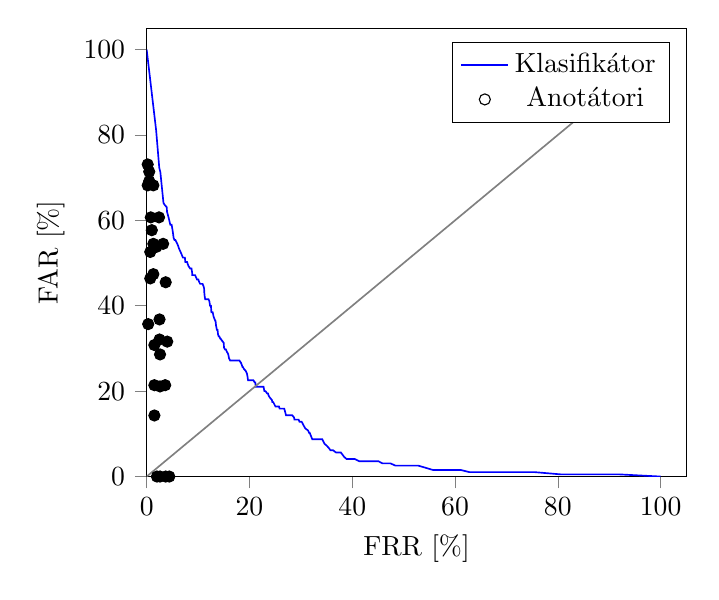
\begin{tikzpicture}

\begin{axis}[
tick align=outside,
tick pos=left,
x grid style={white!69.01960784313725!black},
xlabel={FRR [\%]},
xmin=0, xmax=105,
y grid style={white!69.01960784313725!black},
ylabel={FAR [\%]},
ymin=0, ymax=105,
legend pos=north east,
]

\addplot [semithick, blue]
table {%
0 100
1.84787279759347 81.025641025641
2.44950580146111 72.3076923076923
2.66437473141384 71.2820512820513
2.96519123334766 67.6923076923077
3.26600773528148 64.1025641025641
3.52385045122475 63.5897435897436
3.91061452513966 63.0769230769231
3.95358831113021 62.0512820512821
4.29737859905458 60.5128205128205
4.5981951009884 58.974358974359
4.85603781693167 58.974358974359
5.0709067468844 57.4358974358974
5.24280189084658 55.8974358974359
5.41469703480877 55.3846153846154
5.58659217877095 55.3846153846154
5.80146110872368 54.8717948717949
6.01633003867641 54.3589743589744
6.31714654061023 53.3333333333333
6.70391061452514 52.3076923076923
6.87580575848732 51.7948717948718
7.04770090244951 51.2820512820513
7.26256983240224 51.2820512820513
7.39149119037387 51.2820512820513
7.43446497636442 51.2820512820513
7.52041254834551 50.2564102564103
7.6063601203266 50.2564102564103
7.82122905027933 50.2564102564103
7.86420283626988 50.2564102564103
7.99312419424151 49.7435897435897
8.1650193382037 49.2307692307692
8.46583584013752 48.7179487179487
8.72367855608079 48.7179487179487
8.85259991405243 47.6923076923077
8.85259991405243 47.1794871794872
9.02449505801461 47.1794871794872
9.15341641598625 47.1794871794872
9.41125913192952 47.1794871794872
9.79802320584444 46.1538461538462
9.92694456381607 46.1538461538462
10.0558659217877 46.1538461538462
10.1847872797593 45.6410256410256
10.3996562097121 45.1282051282051
10.5285775676837 45.1282051282051
10.7004727116459 45.1282051282051
10.8723678556081 45.1282051282051
11.0442629995703 44.6153846153846
11.1731843575419 44.1025641025641
11.2161581435324 43.0769230769231
11.3021057155135 42.0512820512821
11.3880532874946 41.5384615384615
11.4740008594757 41.5384615384615
11.5169746454663 41.5384615384615
11.6029222174474 41.5384615384615
11.8607649333906 41.5384615384615
12.0326600773528 41.5384615384615
12.204555221315 41.025641025641
12.3334765792866 40
12.5053717232488 40
12.5053717232488 40
12.5053717232488 40
12.5913192952299 38.4615384615385
12.6342930812205 38.4615384615385
12.8491620111732 38.4615384615385
13.0210571551354 37.4358974358974
13.1929522990976 36.9230769230769
13.3648474430597 36.4102564102564
13.4078212290503 36.4102564102564
13.4937688010314 35.3846153846154
13.6656639449936 34.3589743589744
13.7945853029652 34.3589743589744
13.8805328749463 33.3333333333333
14.0094542329179 32.8205128205128
14.1383755908896 32.8205128205128
14.3102707348517 32.3076923076923
14.3962183068328 32.3076923076923
14.6540610227761 31.7948717948718
14.6970348087667 31.7948717948718
14.9978513107005 31.2820512820513
15.040825096691 30.2564102564103
15.2556940266437 29.7435897435897
15.4275891706059 29.7435897435897
15.5994843145681 29.2307692307692
15.8573270305114 28.7179487179487
16.0292221744736 27.6923076923077
16.2440911044263 27.1794871794872
16.4159862483885 27.1794871794872
16.5449076063601 27.1794871794872
16.8886978942845 27.1794871794872
16.9746454662656 27.1794871794872
17.1035668242372 27.1794871794872
17.3184357541899 27.1794871794872
17.6192522561238 27.1794871794872
17.8341211860765 27.1794871794872
17.9200687580576 27.1794871794872
18.0489901160292 27.1794871794872
18.3068328319725 26.6666666666667
18.349806617963 26.6666666666667
18.6506231198969 25.6410256410256
18.736570691878 25.6410256410256
18.9514396218307 25.1282051282051
18.9944134078212 25.1282051282051
19.3382036957456 24.6153846153846
19.5100988397078 24.1025641025641
19.5960464116889 23.5897435897436
19.7249677696605 22.5641025641026
19.9828104856038 22.5641025641026
20.3266007735281 22.5641025641026
20.5414697034809 22.5641025641026
20.7563386334336 22.5641025641026
21.0141813493769 22.0512820512821
21.1431027073485 22.0512820512821
21.2290502793296 21.025641025641
21.4439192092823 21.025641025641
21.7017619252256 21.025641025641
22.0025784271594 21.025641025641
22.1744735711216 21.025641025641
22.4323162870649 21.025641025641
22.7331327889987 21.025641025641
22.9050279329609 20
23.1198968629136 20
23.4207133648474 19.4871794871795
23.5926085088096 19.4871794871795
23.7215298667813 18.974358974359
23.9793725827245 18.4615384615385
24.3661366566395 17.9487179487179
24.4520842286205 17.4358974358974
24.6239793725827 17.4358974358974
24.8388483025355 16.9230769230769
25.0537172324882 16.4102564102564
25.1826385904598 16.4102564102564
25.4404813064031 16.4102564102564
25.7412978083369 16.4102564102564
25.8702191663086 15.8974358974359
25.9991405242802 15.8974358974359
26.1710356682424 15.8974358974359
26.4288783841856 15.8974358974359
26.77266867211 15.8974358974359
27.1164589600344 14.3589743589744
27.3743016759777 14.3589743589744
27.6751181779115 14.3589743589744
28.0189084658358 14.3589743589744
28.3197249677697 14.3589743589744
28.663515255694 13.8461538461538
28.7494628276751 13.3333333333333
28.9643317576278 13.3333333333333
29.5659647614955 13.3333333333333
29.7378599054577 12.8205128205128
30.1675977653631 12.8205128205128
30.3824666953159 12.3076923076923
30.8551783412119 11.2820512820513
31.413837559089 10.7692307692308
31.5857327030511 10.2564102564103
31.7146540610228 10.2564102564103
32.2303394929093 8.71794871794872
32.6600773528148 8.71794871794872
33.1327889987108 8.71794871794872
33.8203695745595 8.71794871794872
34.1641598624839 8.71794871794872
34.5938977223893 7.69230769230769
35.0666093682853 7.17948717948718
35.4533734422003 6.66666666666667
35.7541899441341 6.15384615384615
36.2698753760206 6.15384615384615
36.8285345938977 5.64102564102564
37.2152986678126 5.64102564102564
37.7739578856897 5.64102564102564
38.4185646755479 4.61538461538462
38.8912763214439 4.1025641025641
39.5358831113021 4.1025641025641
39.922647185217 4.1025641025641
40.4813064030941 4.1025641025641
41.340782122905 3.58974358974359
42.0713364847443 3.58974358974359
42.6729694886119 3.58974358974359
43.1886549204985 3.58974358974359
44.0481306403094 3.58974358974359
45.0795015040825 3.58974358974359
45.8960034379029 3.07692307692308
46.5406102277611 3.07692307692308
47.4430597335625 3.07692307692308
48.3884830253545 2.56410256410256
49.5487752470993 2.56410256410256
50.4941985388913 2.56410256410256
51.2247529007306 2.56410256410256
52.8147829823807 2.56410256410256
54.2758917060593 2.05128205128205
55.6940266437473 1.53846153846154
57.3700042973786 1.53846153846154
59.3467984529437 1.53846153846154
61.1087236785561 1.53846153846154
62.8276751181779 1.02564102564103
65.0623119896863 1.02564102564103
68.1993983669961 1.02564102564103
71.8521701761925 1.02564102564103
75.5479157713795 1.02564102564103
80.5328749462828 0.512820512820513
85.1310700472712 0.512820512820513
91.8349806617963 0.512820512820513
100 0
};
\addlegendentry{Klasifikátor}

\addplot [scatter, only marks, scatter src=explicit symbolic,
          scatter/classes={
            a={mark=o, draw=black, fill=black}
          }
]
table {%
03.00 14.30 a
01.50 21.40 a
00.30 35.70 a
03.60 21.40 a
02.60 28.60 a
00.80 60.70 a
00.70 46.40 a
00.50 71.40 a
02.50 32.10 a
02.40 60.70 a
01.30 47.40 a
02.60 21.10 a
00.70 52.60 a
04.00 31.60 a
02.50 36.80 a
01.50 14.30 a
03.70 00.00 a
02.00 00.00 a
04.40 00.00 a
02.60 00.00 a
00.50 69.20 a
01.50 30.80 a
01.00 57.70 a
00.20 73.10 a
01.90 53.80 a
01.30 68.20 a
03.20 54.50 a
01.30 54.50 a
00.20 68.20 a
03.70 45.50 a
}; \addlegendentry{Anotátori}


\addplot [semithick, gray, forget plot]
table [row sep=\\]{%
0	0 \\
0.50251256281407	0.50251256281407 \\
1.00502512562814	1.00502512562814 \\
1.50753768844221	1.50753768844221 \\
2.01005025125628	2.01005025125628 \\
2.51256281407035	2.51256281407035 \\
3.01507537688442	3.01507537688442 \\
3.51758793969849	3.51758793969849 \\
4.02010050251256	4.02010050251256 \\
4.52261306532663	4.52261306532663 \\
5.0251256281407	5.0251256281407 \\
5.52763819095477	5.52763819095477 \\
6.03015075376884	6.03015075376884 \\
6.53266331658291	6.53266331658291 \\
7.03517587939698	7.03517587939698 \\
7.53768844221105	7.53768844221105 \\
8.04020100502512	8.04020100502512 \\
8.5427135678392	8.5427135678392 \\
9.04522613065327	9.04522613065327 \\
9.54773869346734	9.54773869346734 \\
10.0502512562814	10.0502512562814 \\
10.5527638190955	10.5527638190955 \\
11.0552763819095	11.0552763819095 \\
11.5577889447236	11.5577889447236 \\
12.0603015075377	12.0603015075377 \\
12.5628140703518	12.5628140703518 \\
13.0653266331658	13.0653266331658 \\
13.5678391959799	13.5678391959799 \\
14.070351758794	14.070351758794 \\
14.572864321608	14.572864321608 \\
15.0753768844221	15.0753768844221 \\
15.5778894472362	15.5778894472362 \\
16.0804020100502	16.0804020100502 \\
16.5829145728643	16.5829145728643 \\
17.0854271356784	17.0854271356784 \\
17.5879396984925	17.5879396984925 \\
18.0904522613065	18.0904522613065 \\
18.5929648241206	18.5929648241206 \\
19.0954773869347	19.0954773869347 \\
19.5979899497487	19.5979899497487 \\
20.1005025125628	20.1005025125628 \\
20.6030150753769	20.6030150753769 \\
21.105527638191	21.105527638191 \\
21.608040201005	21.608040201005 \\
22.1105527638191	22.1105527638191 \\
22.6130653266332	22.6130653266332 \\
23.1155778894472	23.1155778894472 \\
23.6180904522613	23.6180904522613 \\
24.1206030150754	24.1206030150754 \\
24.6231155778894	24.6231155778894 \\
25.1256281407035	25.1256281407035 \\
25.6281407035176	25.6281407035176 \\
26.1306532663317	26.1306532663317 \\
26.6331658291457	26.6331658291457 \\
27.1356783919598	27.1356783919598 \\
27.6381909547739	27.6381909547739 \\
28.1407035175879	28.1407035175879 \\
28.643216080402	28.643216080402 \\
29.1457286432161	29.1457286432161 \\
29.6482412060301	29.6482412060301 \\
30.1507537688442	30.1507537688442 \\
30.6532663316583	30.6532663316583 \\
31.1557788944724	31.1557788944724 \\
31.6582914572864	31.6582914572864 \\
32.1608040201005	32.1608040201005 \\
32.6633165829146	32.6633165829146 \\
33.1658291457286	33.1658291457286 \\
33.6683417085427	33.6683417085427 \\
34.1708542713568	34.1708542713568 \\
34.6733668341708	34.6733668341708 \\
35.1758793969849	35.1758793969849 \\
35.678391959799	35.678391959799 \\
36.1809045226131	36.1809045226131 \\
36.6834170854271	36.6834170854271 \\
37.1859296482412	37.1859296482412 \\
37.6884422110553	37.6884422110553 \\
38.1909547738693	38.1909547738693 \\
38.6934673366834	38.6934673366834 \\
39.1959798994975	39.1959798994975 \\
39.6984924623116	39.6984924623116 \\
40.2010050251256	40.2010050251256 \\
40.7035175879397	40.7035175879397 \\
41.2060301507538	41.2060301507538 \\
41.7085427135678	41.7085427135678 \\
42.2110552763819	42.2110552763819 \\
42.713567839196	42.713567839196 \\
43.21608040201	43.21608040201 \\
43.7185929648241	43.7185929648241 \\
44.2211055276382	44.2211055276382 \\
44.7236180904523	44.7236180904523 \\
45.2261306532663	45.2261306532663 \\
45.7286432160804	45.7286432160804 \\
46.2311557788945	46.2311557788945 \\
46.7336683417085	46.7336683417085 \\
47.2361809045226	47.2361809045226 \\
47.7386934673367	47.7386934673367 \\
48.2412060301507	48.2412060301507 \\
48.7437185929648	48.7437185929648 \\
49.2462311557789	49.2462311557789 \\
49.748743718593	49.748743718593 \\
50.251256281407	50.251256281407 \\
50.7537688442211	50.7537688442211 \\
51.2562814070352	51.2562814070352 \\
51.7587939698492	51.7587939698492 \\
52.2613065326633	52.2613065326633 \\
52.7638190954774	52.7638190954774 \\
53.2663316582914	53.2663316582914 \\
53.7688442211055	53.7688442211055 \\
54.2713567839196	54.2713567839196 \\
54.7738693467337	54.7738693467337 \\
55.2763819095477	55.2763819095477 \\
55.7788944723618	55.7788944723618 \\
56.2814070351759	56.2814070351759 \\
56.7839195979899	56.7839195979899 \\
57.286432160804	57.286432160804 \\
57.7889447236181	57.7889447236181 \\
58.2914572864322	58.2914572864322 \\
58.7939698492462	58.7939698492462 \\
59.2964824120603	59.2964824120603 \\
59.7989949748744	59.7989949748744 \\
60.3015075376884	60.3015075376884 \\
60.8040201005025	60.8040201005025 \\
61.3065326633166	61.3065326633166 \\
61.8090452261306	61.8090452261306 \\
62.3115577889447	62.3115577889447 \\
62.8140703517588	62.8140703517588 \\
63.3165829145729	63.3165829145729 \\
63.8190954773869	63.8190954773869 \\
64.321608040201	64.321608040201 \\
64.8241206030151	64.8241206030151 \\
65.3266331658291	65.3266331658291 \\
65.8291457286432	65.8291457286432 \\
66.3316582914573	66.3316582914573 \\
66.8341708542713	66.8341708542713 \\
67.3366834170854	67.3366834170854 \\
67.8391959798995	67.8391959798995 \\
68.3417085427136	68.3417085427136 \\
68.8442211055276	68.8442211055276 \\
69.3467336683417	69.3467336683417 \\
69.8492462311558	69.8492462311558 \\
70.3517587939699	70.3517587939699 \\
70.8542713567839	70.8542713567839 \\
71.356783919598	71.356783919598 \\
71.859296482412	71.859296482412 \\
72.3618090452261	72.3618090452261 \\
72.8643216080402	72.8643216080402 \\
73.3668341708543	73.3668341708543 \\
73.8693467336683	73.8693467336683 \\
74.3718592964824	74.3718592964824 \\
74.8743718592965	74.8743718592965 \\
75.3768844221105	75.3768844221105 \\
75.8793969849246	75.8793969849246 \\
76.3819095477387	76.3819095477387 \\
76.8844221105528	76.8844221105528 \\
77.3869346733668	77.3869346733668 \\
77.8894472361809	77.8894472361809 \\
78.391959798995	78.391959798995 \\
78.894472361809	78.894472361809 \\
79.3969849246231	79.3969849246231 \\
79.8994974874372	79.8994974874372 \\
80.4020100502512	80.4020100502512 \\
80.9045226130653	80.9045226130653 \\
81.4070351758794	81.4070351758794 \\
81.9095477386935	81.9095477386935 \\
82.4120603015075	82.4120603015075 \\
82.9145728643216	82.9145728643216 \\
83.4170854271357	83.4170854271357 \\
83.9195979899497	83.9195979899497 \\
84.4221105527638	84.4221105527638 \\
84.9246231155779	84.9246231155779 \\
85.4271356783919	85.4271356783919 \\
85.929648241206	85.929648241206 \\
86.4321608040201	86.4321608040201 \\
86.9346733668342	86.9346733668342 \\
87.4371859296482	87.4371859296482 \\
87.9396984924623	87.9396984924623 \\
88.4422110552764	88.4422110552764 \\
88.9447236180904	88.9447236180904 \\
89.4472361809045	89.4472361809045 \\
89.9497487437186	89.9497487437186 \\
90.4522613065326	90.4522613065326 \\
90.9547738693467	90.9547738693467 \\
91.4572864321608	91.4572864321608 \\
91.9597989949749	91.9597989949749 \\
92.4623115577889	92.4623115577889 \\
92.964824120603	92.964824120603 \\
93.4673366834171	93.4673366834171 \\
93.9698492462311	93.9698492462311 \\
94.4723618090452	94.4723618090452 \\
94.9748743718593	94.9748743718593 \\
95.4773869346734	95.4773869346734 \\
95.9798994974874	95.9798994974874 \\
96.4824120603015	96.4824120603015 \\
96.9849246231156	96.9849246231156 \\
97.4874371859296	97.4874371859296 \\
97.9899497487437	97.9899497487437 \\
98.4924623115578	98.4924623115578 \\
98.9949748743718	98.9949748743718 \\
99.4974874371859	99.4974874371859 \\
100	100 \\
};

\end{axis}

\end{tikzpicture}}
    \caption{Fonéma \textipa{/t/}}
\end{subfigure}\\
\caption{FAR a FRR určené po dvojiciach anotátorov, kde anotácie jedného anotátora v~dvojici sú považované za referenčné. Pre porovnanie je taktiež uvedená krivka LR GOP metódy s~najlepšími výsledkami.}
\label{fig:inter-judge}
\end{figure}